\documentclass{article}

% if you need to pass options to natbib, use, e.g.:
%     \PassOptionsToPackage{numbers, compress}{natbib}
% before loading neurips_2024


% ready for submission
\usepackage[final]{neurips_2024}


% to compile a preprint version, e.g., for submission to arXiv, add add the
% [preprint] option:
%     \usepackage[preprint]{neurips_2024}


% to compile a camera-ready version, add the [final] option, e.g.:
%     \usepackage[final]{neurips_2024}

% to avoid loading the natbib package, add option nonatbib:
%    \usepackage[nonatbib]{neurips_2024}
\usepackage{graphicx} % Required for including images
\usepackage{subcaption} % Required for subfigure (if using subfigure)
\usepackage{float}

\usepackage[utf8]{inputenc} % allow utf-8 input
\usepackage[T1]{fontenc}    % use 8-bit T1 fonts
\usepackage{hyperref}       % hyperlinks
\usepackage{url}            % simple URL typesetting
\usepackage{booktabs} 
\usepackage{amsmath, amssymb}
% professional-quality tables
\usepackage{amsfonts}       % blackboard math symbols
\usepackage{nicefrac}       % compact symbols for 1/2, etc.
\usepackage{microtype}      % microtypography
\usepackage{xcolor}         % colors


\title{Bayesian Physics-Informed Neural Networks}


% The \author macro works with any number of authors. There are two commands
% used to separate the names and addresses of multiple authors: \And and \AND.
%
% Using \And between authors leaves it to LaTeX to determine where to break the
% lines. Using \AND forces a line break at that point. So, if LaTeX puts 3 of 4
% authors names on the first line, and the last on the second line, try using
% \AND instead of \And before the third author name.


\author{%
  Anouk Ruer -- Ruben Ifrah -- Pénélope Forcioli \\
}


\begin{document}


\maketitle

\begin{abstract}
In this report, we reproduce and analyze the main methodology and empirical findings of the paper \cite{Yang_2021}. We then propose three extensions. First, we introduce additional quantitative metrics to systematically evaluate predictive uncertainty and calibration across different models. Second, we extend the B-PINN framework by treating the observational noise level as an unknown parameter and inferring it jointly with the network parameters through HMC. Third, we investigate the theoretical infinite-width limit of Bayesian PINNs and show that it converges to a Physics-Informed Gaussian Process.
\end{abstract}


\section{Methodology}

\subsection{B-PINNs: Bayesian Physics-informed Neural Networks}
The paper considers a general PDE of the form : 

\[ N_x(u; \lambda) = f \quad \text{on the domain} \quad D ; \qquad
B_x(u; \lambda) = b \quad  \text{on the boundary} \quad \Gamma.
\]

Where $N_x$ is a differential operator (possibly nonlinear), $u(x)$ is the unknwon solution, $\lambda$ is a vector of PDE parameters, $f$ is the forcing term and $B_x$ is the boundary condition operator. The distinction between forward and inverse problems is: in forward problem, $\lambda$ is known and you want to find $u$ ; in inverse problem, $\lambda$ is also unknown and must be inferred from data jointly with $u$.

The available data $D$ consists of scattered noisy sensor measurements of $u, f,$ and $b$:
$D = D_u \cup D_f \cup D_b$.
A key modeling assumption is that all observations are independently Gaussian distributed around the true hidden value, with known standard deviations $\sigma$. This assumption directly determines the structure of the likelihood function.

\subsection{Prior for Bayesian Physics-informed Neural Networks}

The solution $u(x)$ is represented by a surrogate model $\tilde{u}(x; \theta)$, where $\theta$ collects all weights and biases of a fully connected neural network with L hidden layers : 

$$z_l = \psi(w_{l_{-1}} z_{l_{-1}} + b_{l_{-1}})$$

with $\psi$ the activation function (the hyperbolic tangent function in our case). Once $\tilde{u}$ is defined, the PDE constraint is used to derive: $f(x; \theta) = N_x(\tilde{u}; \lambda)$ the predicted forcing term via automatic differentiation. And $\tilde{b}(x; \theta) = B_x(\tilde{u}; \lambda)$ the predicted boundary values. This is the physics-informed part: the neural network doesn't just fit data, it must also satisfy the PDE structure through its derivatives. This is what distinguishes B-PINNs from BNNs, which only model observational data. 


A gaussian prior is placed independently on each component of $\theta$. The paper notes that as the network width goes to infinity, this induces a Gaussian process prior on $\tilde{u}(x)$. However, for finite-width networks, higher-order derivatives of $\tilde{u}$ are not necessarily Gaussian processes, which is particularly relevant since the PDE constraints involve such derivatives. Under these assumptions, the likelihood is thus as follows:

\begin{align*}
    P(D|\theta) &= P(D_u|\theta) · P(D_f|\theta) · P(D_b|\theta)
\end{align*}


\subsection{Posterior sampling approaches for Bayesian Physics-informed Neural Networks}
 
By Bayes' theorem : $P(\theta|D) \propto P(D|\theta) · P(\theta)$. The normalizing constant $P(D)$ is analytically intractable, so only the unnormalized posterior is available. Inference therefore requires either sampling or approximation methods. In the case of inverse problems, $\lambda$ gets its own prior $P(\lambda)$ and the joint posterior $P(\theta, \lambda|D)$ is estimated instead. The paper proposes two approaches to sample from the posterior.

\paragraph{Hamiltonian Monte Carlo (HMC) method} is an MCMC method that uses Hamiltonian dynamics to propose efficient moves in parameter space, avoiding the random walk behavior of simpler MCMC methods \cite{Brooks_2011}. HMC introduces an auxiliary momentum variable $r$ to define a Hamiltonian: $H(\theta, r) = U(\theta) + \frac{1}{2} r^T M^{-1} r$ where the potential energy $U(\theta) = - ln P(D|\theta) - ln P(\theta)$  is the negative log-posterior of the model. The dynamics evolve according to Hamilton’s equations, which are numerically integrated using the leapfrog scheme. Because discretization introduces approximation error, a final Metropolis–Hastings correction step ensures that the Markov chain preserves the desired posterior distribution. Under standard regularity conditions, HMC produces asymptotically exact samples from the posterior distribution.


\paragraph{Variational Inference (VI) method} Rather than drawing posterior samples as in HMC, VI recasts Bayesian inference as an optimization problem. The posterior distribution $P(\theta |D)$ is approximated by a parametric distribution $Q(\theta ; \zeta)$ chosen from a tractable family. The variational parameters 
$\zeta$ are obtained by minimizing the Kullback–Leibler divergence 
$KL(Q(\theta;\zeta) || P(\theta|D))$, which is equivalent to minimize 
$E_{\theta \sim Q} [ln Q(\theta ; \zeta) - ln P(\theta) - ln P(D| \theta)]$. 
The family chosen is a fully factorizable Gaussian, each parameter $\theta_i$ gets its own independent Gaussian with trainable mean $\zeta_{\mu,i}$ and standard deviation parameterized via a softplus transform $log(1 + exp( \zeta_{\rho,i}))$ to ensure positivity. A reparameterization trick allows gradients to flow through the sampling operation, and Adam is used to optimize $\zeta$.
A limitation of this appraoch is the factorized Gaussian distribution assumption, wich enforces independence between all parameters. In a neural network posterior, weights are often strongly correlated, so this family is fundamentally too restrictive. Leading to underestimated posterior variance and degraded uncertainty quantification.

\subsection{Empirical Evaluation}

To evaluate the B-PINN framework, the paper conducts a systematic comparison across five approaches. The standard PINN serves as the baseline, producing point estimates with no uncertainty quantification. B-PINN-HMC and B-PINN-VI both embed the PINN structure within a Bayesian framework, using a BNN as prior and a Gaussian likelihood for noisy observations. Dropout is included as a non-Bayesian uncertainty baseline, tested at rates of 1\% and 5\%: the network is trained with neurons randomly zeroed at each step, and at inference time dropout is kept active so that $M=10 000$ stochastic forward passes yiels an empirical mean and standard deviation as uncertainty estimate. They start with a comparison of BNNs and NNs on a function regression problem. The models are then tested on two forward PDE problems: the 1D Poisson equation and the 2D nonlinear Allen-Cahn equation, and then on two inverse problems: the 1D diffusion-reaction system with nonlinear source term and the 2D nonlinear diffusion-reaction system problem. BNNS and PINNs are directly compared on  the 1D diffusion-reaction system with nonlinear source term inverse problem.

Lastly, the authors investigate whether a lighter surrogate model could replace the BNN while remaining the same Bayesian framework. The used the truncated Karhunen-Loève (KL) expansion. The core idea is to decompose the unknown function $u(x)$ into a sum of deterministic eigenfuntions weighted by a random scalar function scalar coefficients : $\tilde{u}(x; \theta) = \mu(x) + \sum^n_{i=1} \sqrt{\alpha_i}\psi_i(x)\theta_i$, where the eigenfunctions $\psi_i$  and eigenvalues $\alpha_i$​ are derived from a prescribed covariance kernel, and $\theta = (\theta_1, \dots, \theta_n)
$ are the unknown parameters to infer. The KL-expansion only has 20 parameters, making posterior sampling much cheaper. They test it paired with HMC and with  a deep normalizing flow (DNF) on the same problems (function regression, forward and inverse PDEs in 1D and 2D) under two noise levels ($\sigma$ = 0.01 and $\sigma$ = 0.1).

\section{Key Findings of the paper}
\subsection{B-PINN-HMC vs. B-PINN-VI vs. Dropout}
\paragraph{B-PINN-HMC has better performances} Across all experiments B-PINN-HMC consistenly delivers the most reliable results. Its predictive means are close to the exact solution and its uncertainty estimates behave correctly : it increases as the noise scale increases and the true solution almost always lies within the two standard deviation confidence interval. In inverse problems, predictions for the unknown parameter kk
k are highly accurate, with errors below 5\% even at high noise, confirming the Bayesian framework's ability to regularize against overfitting where standard PINNs degrade significantly.


\paragraph{VI fails} On the linear 1D Poisson forward problem, B-PINN-VI completely fails to produce any meaningful prediction for u. On the nonlinear cases it partially recovers, producing means closer to the exact solution, but its uncertainty quantification remains unreliable. Even at boundary points where observations are directly provided, B-PINN-VI still reports large uncertainty, likely because it restricts the posterior approximation to a factorizable Gaussian family that's too simple to capture the true distribution.

\paragraph{Dropout is wrong} Despite producing means that appear to fit the training data, dropout predictions diverge significantly from the true solution. Its uncertainty estimates are essentially insensitive to the noise scale across all tested cases, and in the 2D Allen-Cahn problem errors exceed 50\% in parts of the domain while remaining outside the two-standard-deviation bounds, making dropout both inaccurate and poorly calibrated. The impact of varying noise scales on the resulting standard deviations was negligible, which demonstrates that dropout fails to properly account for or quantify uncertainty when processing noisy data.

\paragraph{B-PINN-HMC outperforms PINNs under large noise} At low noise ($\sigma$ = 0.01): both methods perform comparably, with PINNs predicting k = 0.705 vs. exact 0.7. At high noise ($\sigma$ = 0.1): PINNs overfits, predicting k = 0.591, while B-PINN-HMC gives k = 0.665 with a meaningful uncertainty estimate. So the Bayesian framework provides a regularization against overfitting.

\paragraph{Computational cost} The authors also conduct a brief comparison of the cost. For the specific inverse problem, the Bayesian approach only doubled the computation time, which the authors consider a "relatively small increase" given the extra information provided. They still caution that this 2x time difference is not a fixed ratio. As the complexity of the task grows, the "cost gap" will widen.

\subsection{Truncated Karhunen-Loeve expansion}
Both KL-HMC and KL-DNF achieve accuracy comparable to B-PINN-HMC: predicted means align closely with exact solutions, errors remain bounded within two standard deviations, and uncertainty grows in proportion with noise scale. KL-HMC is significantly faster than B-PINN-HMC ($\sim$4 vs $\sim$20 minutes) thanks to its smaller parameter space. DNF is far more expensive to train ($\sim$1 day) but allows fast independent sampling once training is complete. The key limitation of the KL approach is that its eigenfunctions must be precomputed from a known covariance kernel, and the number of terms required to retain sufficient energy grows rapidly with the input dimension, the so-called curse of dimensionality. BNNs, by contrast, are known to handle high-dimensional function approximation efficiently.


\section{Extensions}

\subsection{Metrics and empirical envaluation}


The authors of \cite{Yang_2021} mostly evaluate B-PINNs and PINNs based on graphical results rather than metric-based computations. 
We therefore explored which metrics could be used to evaluate B-PINNs beyond simple visual inspection, and that would allow a direct comparison with standard PINNs. However, the main advantage of B-PINNs lies in their ability to quantify uncertainty. Evaluating only the difference between predictive means largely discards this benefit. A more principled alternative would be to endow standard PINNs with an uncertainty estimate and compare both models using uncertainty-aware metrics. In the paper, the authors use dropout, and in classical neural networks, this is often done by training ensembles and using their empirical mean and variance \cite{lakshminarayanan2017simplescalablepredictiveuncertainty}. While this approach could be extended to PINNs, we do not pursue it in this work. Hence, while we evaluate standard PINNs using classical deterministic metrics like the relative L2 norm ($\text{Relative } L_2 = \frac{||u_{pred} - u_{true}||_2}{||u_{true}||_2}$), we assess Bayesian PINNs through a combination of qualitative checks and quantitative uncertainty measures. First, we compute the relative $L^2$ norm of the mean. 

\paragraph{Prediction Interval Coverage Probability (PICP)}
Specifically, we first visually verify whether the true solution falls entirely within the $\pm 2\sigma$ confidence interval of the predictive mean, which we then formalize using the PICP \cite{picp_mpiw} to measure the exact percentage of true data points captured within these bounds across the test domain. For $N$ test points, if your model predicts a lower bound $L_i$ and an upper bound $U_i$ for each point $i$, the PICP is:

$$\text{PICP} = \frac{1}{N} \sum_{i=1}^{N} c_i$$

Where $c_i = 1$ if the true value is inside the bounds ($L_i \le y_{true, i} \le U_i$) and $c_i = 0$ if it falls outside the bounds.

\paragraph{Mean Prediction Interval Width (MPIW)}
To ensure these intervals are practically informative rather than massive and vague, we also calculate the MPIW \cite{picp_mpiw}, optimizing for the tightest possible bands that still maintain our target PICP.  For $N$ test points, where $U_i$ is your upper bound and $L_i$ is your lower bound, the MPIW is just the average distance between them:

$$\text{MPIW} = \frac{1}{N} \sum_{i=1}^{N} (U_i - L_i)$$

\paragraph{ Negative Log-Likelihood (NLL)} Finally, we compute the NLL \cite{NLL}, that simultaneously evaluates the raw accuracy of the predictive mean and the calibration of the uncertainty spread, effectively penalizing models that are "confidently wrong."

$$\text{NLL} = \frac{1}{N} \sum_{i=1}^{N} \left( \frac{\log(2\pi\sigma_i^2)}{2} + \frac{(y_i - \mu_i)^2}{2\sigma_i^2} \right)$$

where $N$ is the total number of points in the test set, $y_i$ is the true, exact solution at point $i$, $\mu_i$ is the mean prediction the B-PINN makes at point $i$  and $\sigma_i^2$ its variance.
 
\paragraph{Expected Calibration Error and Reliability Diagrams \cite{ECE}}
A Reliability Diagram partitions the predictive confidence into $M$ bins and compares the mean predicted confidence within each bin to the actual observed accuracy (fraction of true values falling within that confidence interval). For a perfectly calibrated B-PINN, the diagram follows a identity line where $x=y$. Quantitatively, the ECE summarizes this deviation by calculating the weighted average difference between the observed accuracy ($acc(B_m)$) and the predicted confidence ($conf(B_m)$) across all bins:$$ECE = \sum_{m=1}^{M} \frac{|B_m|}{N} \left| acc(B_m) - conf(B_m) \right|$$


\subsection{B-PINNs with unknown noise}
\subsubsection{Adding a prior on the noise in forward and inverse problems}
In the framework of this paper the noise levels of the sensors ($\sigma_b$ and $\sigma_f$) are known. This is not a realistic assumption as with real-life measurements, it is usually not possible to know precisely this noise. We thus propose to relax this assumption for $\sigma_f$, while keeping $\sigma_b$ fixed. 
The justification for this is statistical : with only $N_b = 2$ boundary observations, the posterior $\sigma_b$ would be almost entirely determined by the prior rather than the data as the likelihood contribution from two points is too weak to meaningfully inform $\sigma_b$. 
Because in our experiment we chose to not include any interior measurement ($\mathcal{D}_u = \emptyset$), the likelihood can be written $P(\mathcal{D}|\theta, \sigma_f) = P(\mathcal{D}_f|\theta, \sigma_f) P(\mathcal{D}_b|\theta)$. To implement this joint inference, we augment the HMC parameter vector to include the unknown noise scale alongside the neural network weights $\theta$. Because standard HMC operates over unconstrained real-valued spaces ($\mathbb{R}$) but a standard deviation must be strictly positive ($\sigma_f > 0$), we perform a change of variables and sample in log-space: $\psi = \log \sigma_f$. We then recover $\sigma_f = \exp(\psi)$ inside the likelihood evaluation. This continuous reparameterization naturally enforces positivity without requiring complex constrained optimization boundaries, allowing the standard leapfrog HMC sampler to be utilized without modification.  Note that We use a log-normal prior. 
Critically, because $\sigma_f$ is now a dynamically updated variable rather than a fixed constant, the normalization coefficient of the Gaussian distribution can no longer be dropped as a constant. The log-likelihood of the forcing term must explicitly retain this variance penalty:

$$\log P(\mathcal{D}_f | \theta, \psi) \propto -N_f \psi - \frac{SSE_f(\theta)}{2 \exp(2\psi)}$$

where $N_f$ is the number of collocation points, and $SSE_f(\theta)$ is the sum of squared  residuals, $\sum_{i=1}^{N_f} (\tilde{f}(x^{(i)}_f ; \theta) - \bar{f^{i}})^2$. 

 Although we will not explore this extension as much, we note for completeness how to extend this idea to inverse problems. The principle is virtually the same,  the HMC parameter vector is again augmented to include the noise. Nevertheless, unlike the forward problem where $\sigma_f$ was inferred, we in this case would need to keep it fixed and infer $\sigma_u$ instead, i.e the interior state measurement noise. The rationale for this shift is one of identifiability. Indeed, if we were to infer the PDE residual noise ($\sigma_f$) alongside $k$, the model would face an ambiguous task: it could artificially inflate $\sigma_f$ to excuse large errors in the physics, completely failing to identify the true value of $k$. 
\subsubsection{Experimental results}
 We tested this extension on the 1D Poisson equation ($\lambda u_{xx} = f(x)$, $\lambda=0.01$) using 80 collocation points for the forcing term. All models (PINN, B-PINN, and Dropout-PINN) shared a fully connected architecture with two 50-neuron hidden layers and Tanh activations; the Dropout-PINN additionally applied a 1\% or 5\% dropout rate per hidden layer, estimating uncertainty via 10,000 Monte Carlo forward passes at prediction time. We assigned a standard normal prior ($\mathcal{N}(0,1)$) to all network weights, with remaining hyperparameters detailed in Tables \ref{tab:hp} and \ref{tab:hp2}. Testing under two noise regimes ($\sigma_u = \sigma_f \in \{0.1, 0.01\}$), we employed a log-normal prior when inferring the noise. Specifically, for the 0.1 noise case, this prior had a mean of 0 and variance of 0.5, with HMC initialized at $\sigma=1$; for the 0.01 case, both the prior mean and HMC initialization were shifted to $e^{-2.3}$ while maintaining the 0.5 variance. These two settings are important so that our initial guess is not too far from the truth, which would be the case in real life settings as we usually know the order of the noise approximately, but also not too close to properly test our algorithm. 

\begin{table}[h]
\centering
\footnotesize
\begin{tabular}{|c|c|c|c|c|c|}
\hline
 & B-PINN & B-PINN (unknown noise)  & PINN & Dropout -5\% & Dropout - 1\%  \\
\hline
Relative $L^2$ norm & 0.2952  & 0.2251  &   0.4338 & 0.3644 &0.3713 \\
\hline
PICP( \%) & 92.60 & 100 & - & 95.50 & 54.00 \\
\hline
MPIW & 0.6465 & 0.7137 & - & 0.7864 & 0.4048 \\
\hline
NLL & -0.3885 & -0.7345 & - & -0.2677 & 0.3478 \\
\hline
ECE &  0.1307 & 0.1016 & -  & 0.0374 & 0.3090 \\
\hline
\end{tabular}
\caption{\footnotesize Metrics for the 1D poisson equation forward problem with measurement noise 0.1}
\label{tab:5x5}
\end{table}

\begin{figure}[h]
\centering
% Première ligne : PINN et BPINN
\begin{subfigure}{0.3\textwidth}
    \centering
    
\includegraphics[width=\linewidth]{Figures/1D poisson sigma=0.1/PINN.png}
    \caption{}
    \label{fig:image2}
\end{subfigure}
\begin{subfigure}{0.3\textwidth}
    \centering
    
\includegraphics[width=\linewidth]{Figures/1D poisson sigma=0.1/BPINN.png}
    \caption{}
    \label{fig:image1}
\end{subfigure}
\begin{subfigure}{0.3\textwidth}
    \centering
        
\includegraphics[width=\linewidth]{Figures/1D poisson sigma=0.1/HBPINN.png}
    \caption{}
    \label{fig:image3}
\end{subfigure}
\hfill\begin{subfigure}{0.3\textwidth}
    \centering
    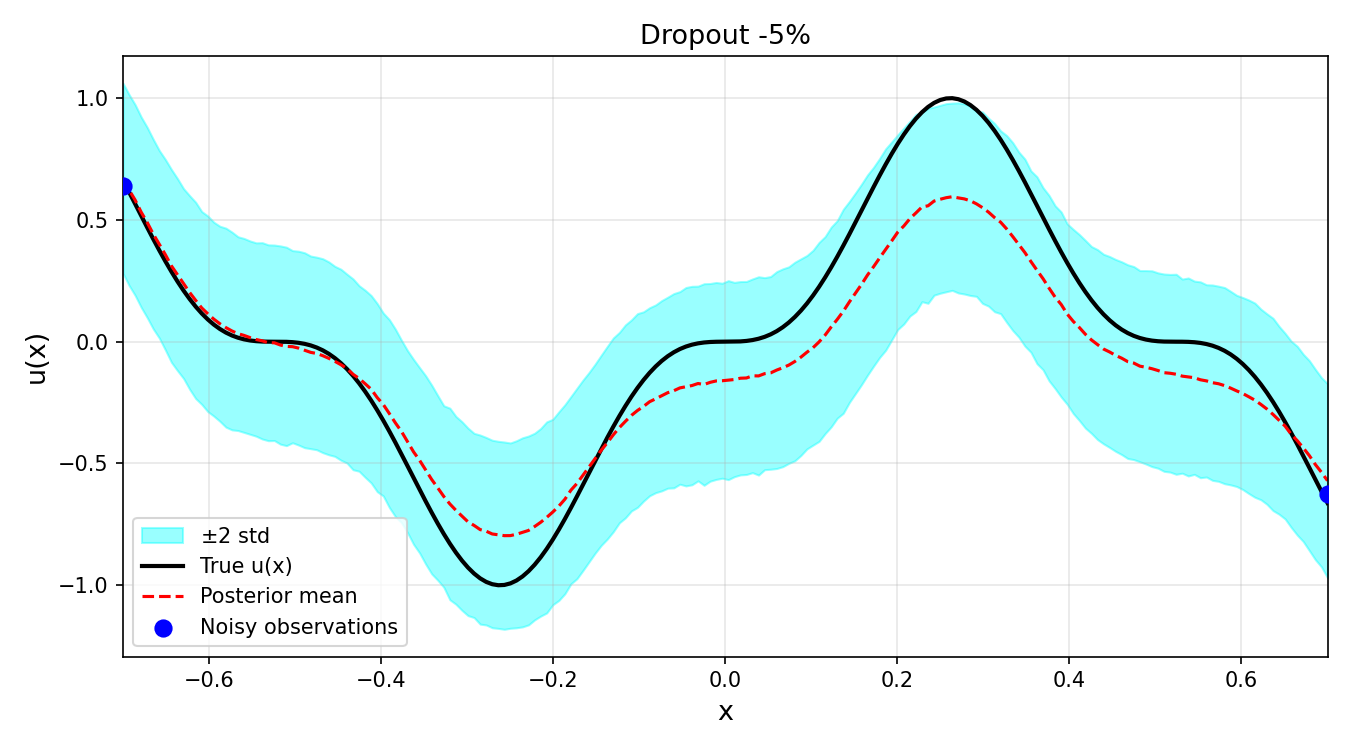
\includegraphics[width=\linewidth]{Figures/dropout/dropout_5_1.png}
    \caption{}
    \label{fig:drop}
\end{subfigure}
\begin{subfigure}{0.3\textwidth}
    \centering
      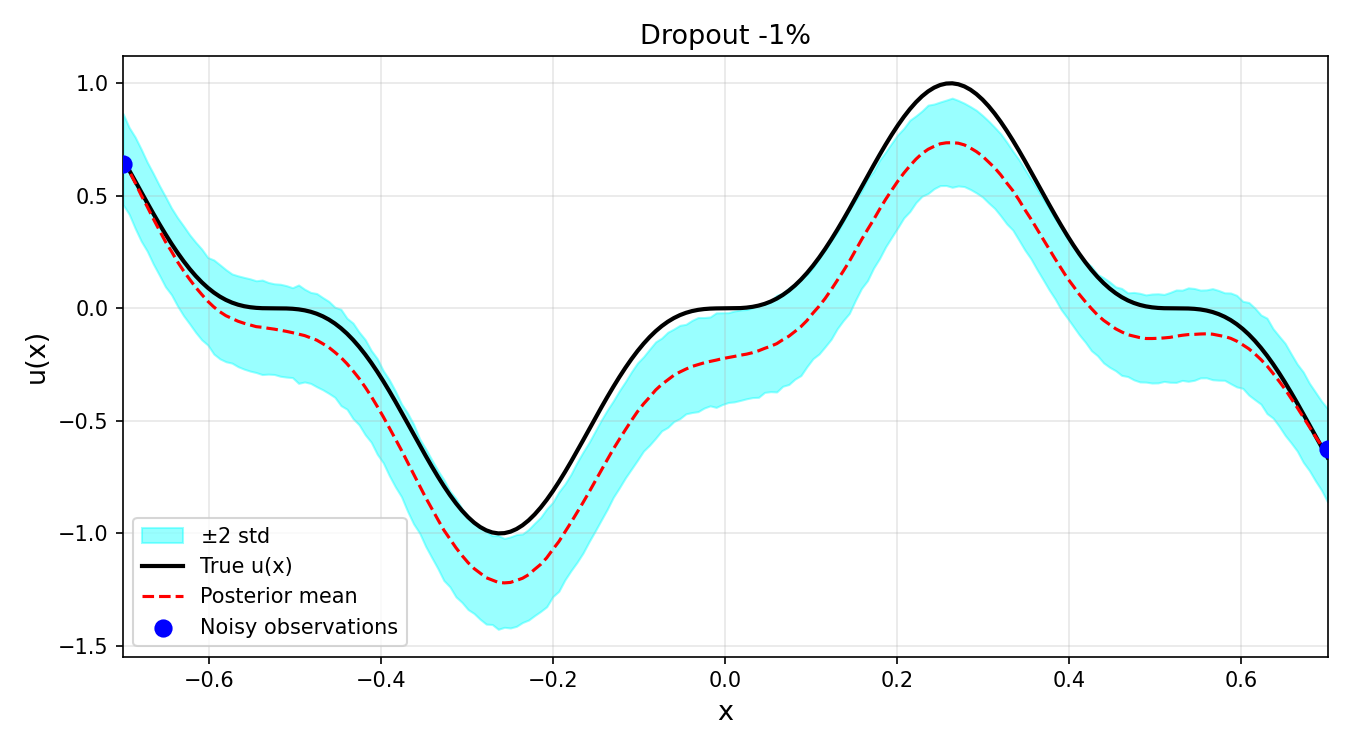
\includegraphics[width=\linewidth]{Figures/dropout/dropout_1_1.png}
    \caption{}
    \label{fig:drop}
\end{subfigure}
\caption{\footnotesize 1D linear Poisson equation- forward problem: predicted u from different methods with noise scale $\epsilon_f \sim \mathcal{N}(0,0.1^2)$ and $\epsilon_b \sim \mathcal{N}(0,0.1^2)$. (c) B-PINN with prior on $\sigma_f$.}
\label{fig:noise01}
\end{figure}

\begin{figure}[h]
\centering
\begin{subfigure}{0.24\textwidth} % Adjust width to fit three images
    \centering
    
\includegraphics[width=\linewidth]{Figures/1D poisson sigma=0.1/BPINN_reliability.png}
    \caption{}
    \label{fig:image1}
\end{subfigure}
\begin{subfigure}{0.24\textwidth} % Adjust width to fit three images
    \centering
    
\includegraphics[width=\linewidth]{Figures/1D poisson sigma=0.1/HBPINN_reliability.png}
    \caption{\footnotesize Unknown noise}
    \label{fig:image2}
\end{subfigure}
\begin{subfigure}{0.24\textwidth} % Adjust width to fit three images
    \centering
    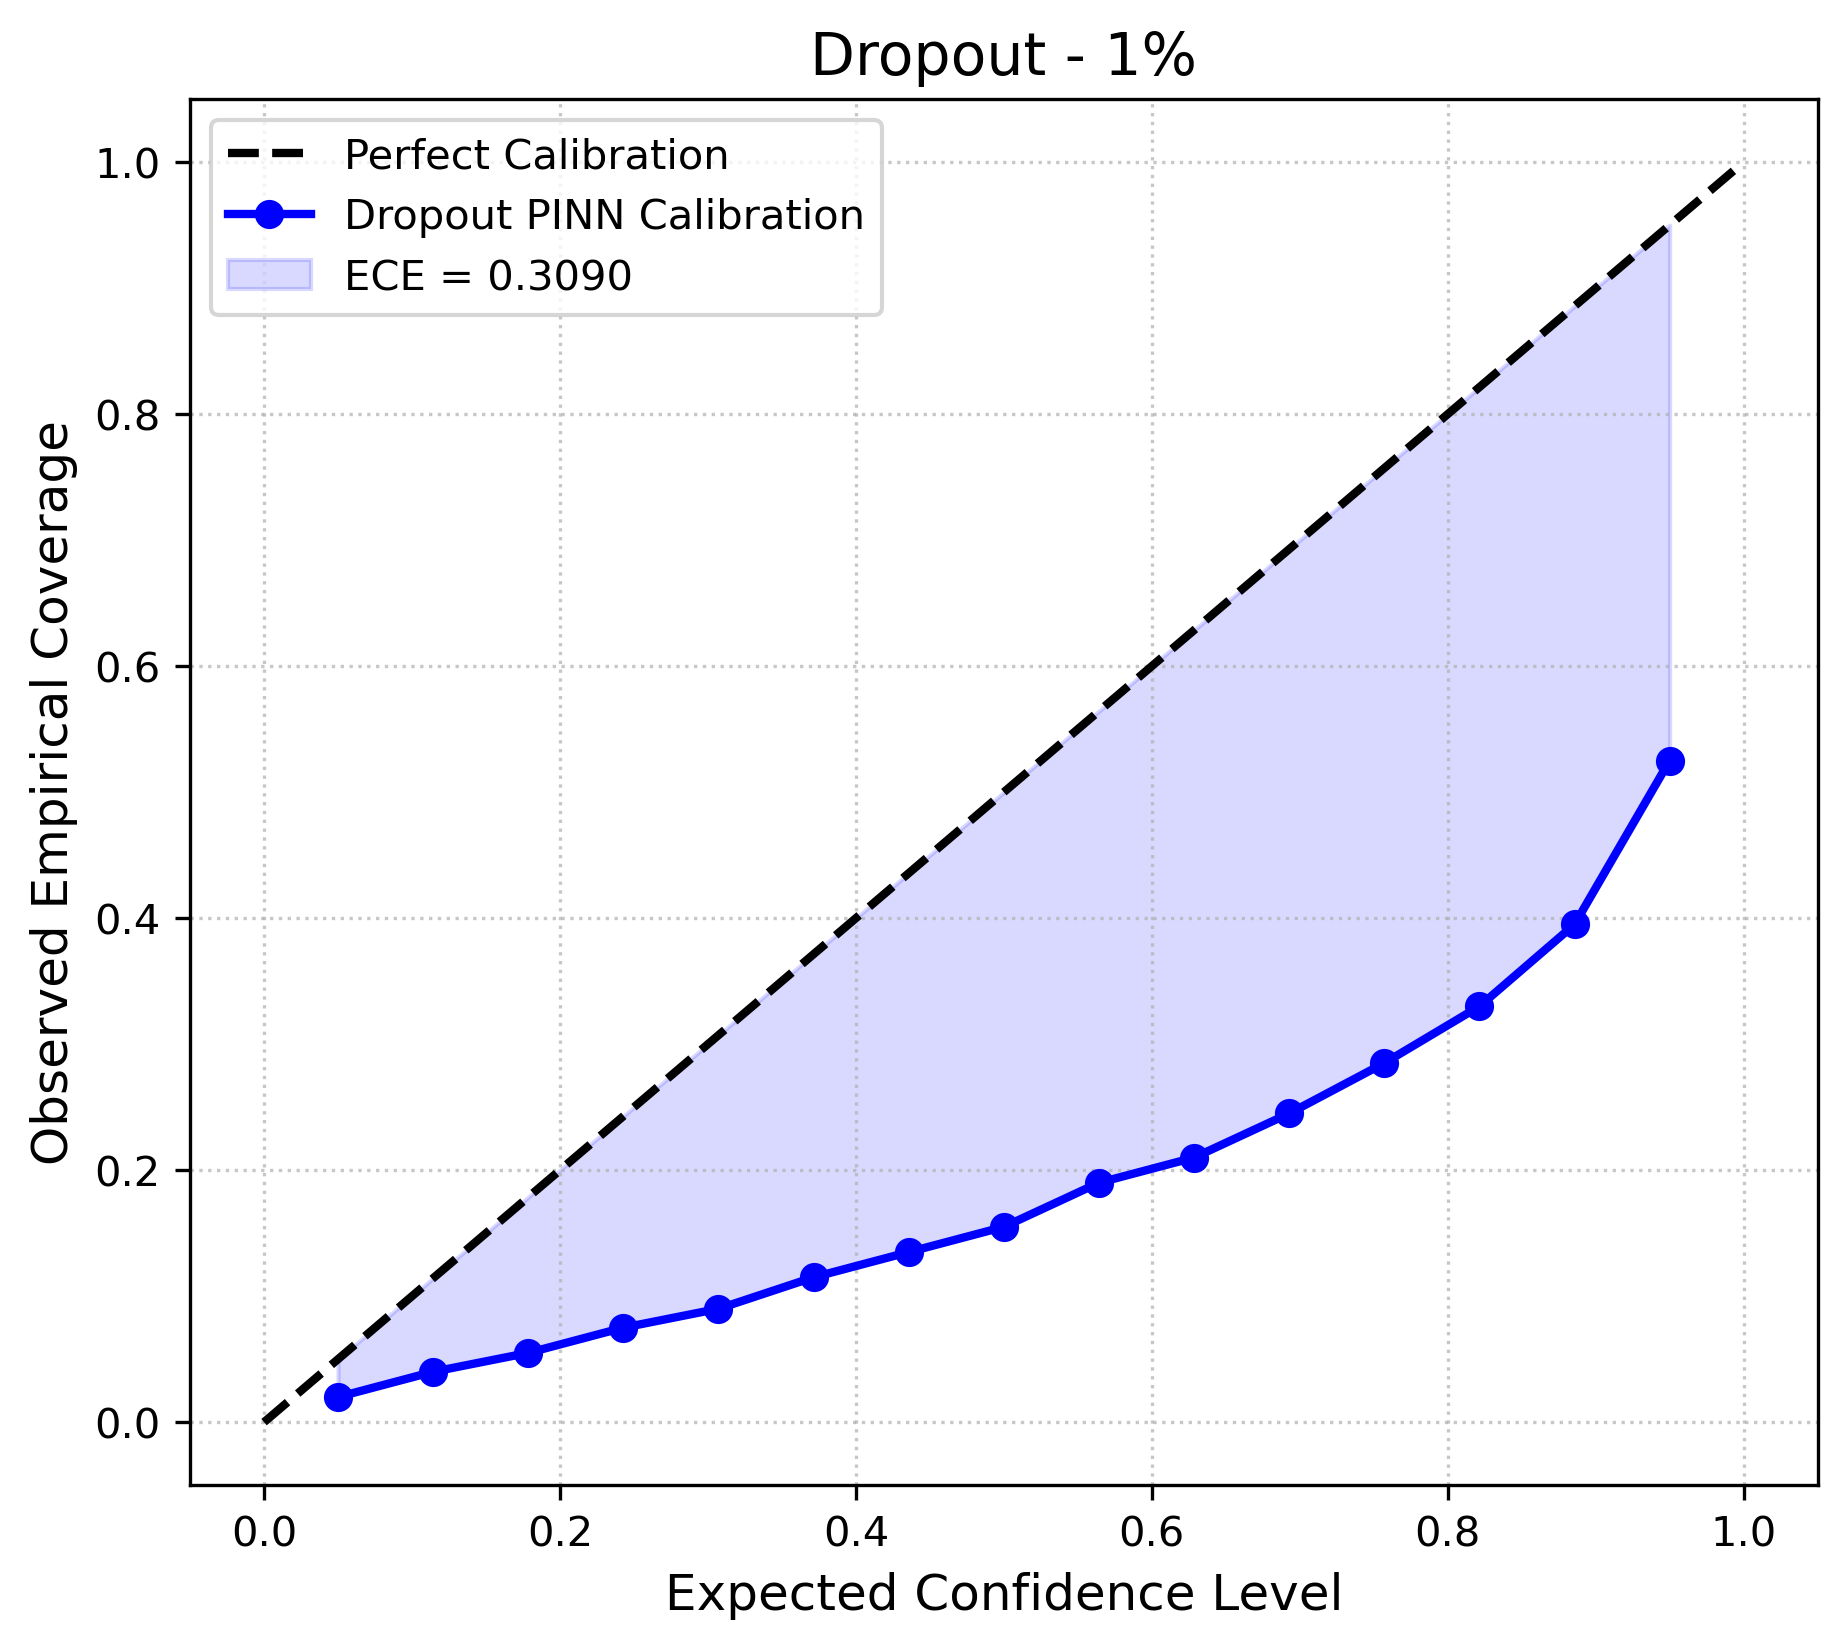
\includegraphics[width=\linewidth]{Figures/dropout/dropout_reliability_1_1.png} % Replace with your third image file
    \caption{}
    \label{fig:image3}
\end{subfigure}
\begin{subfigure}{0.24\textwidth} 
    \centering
    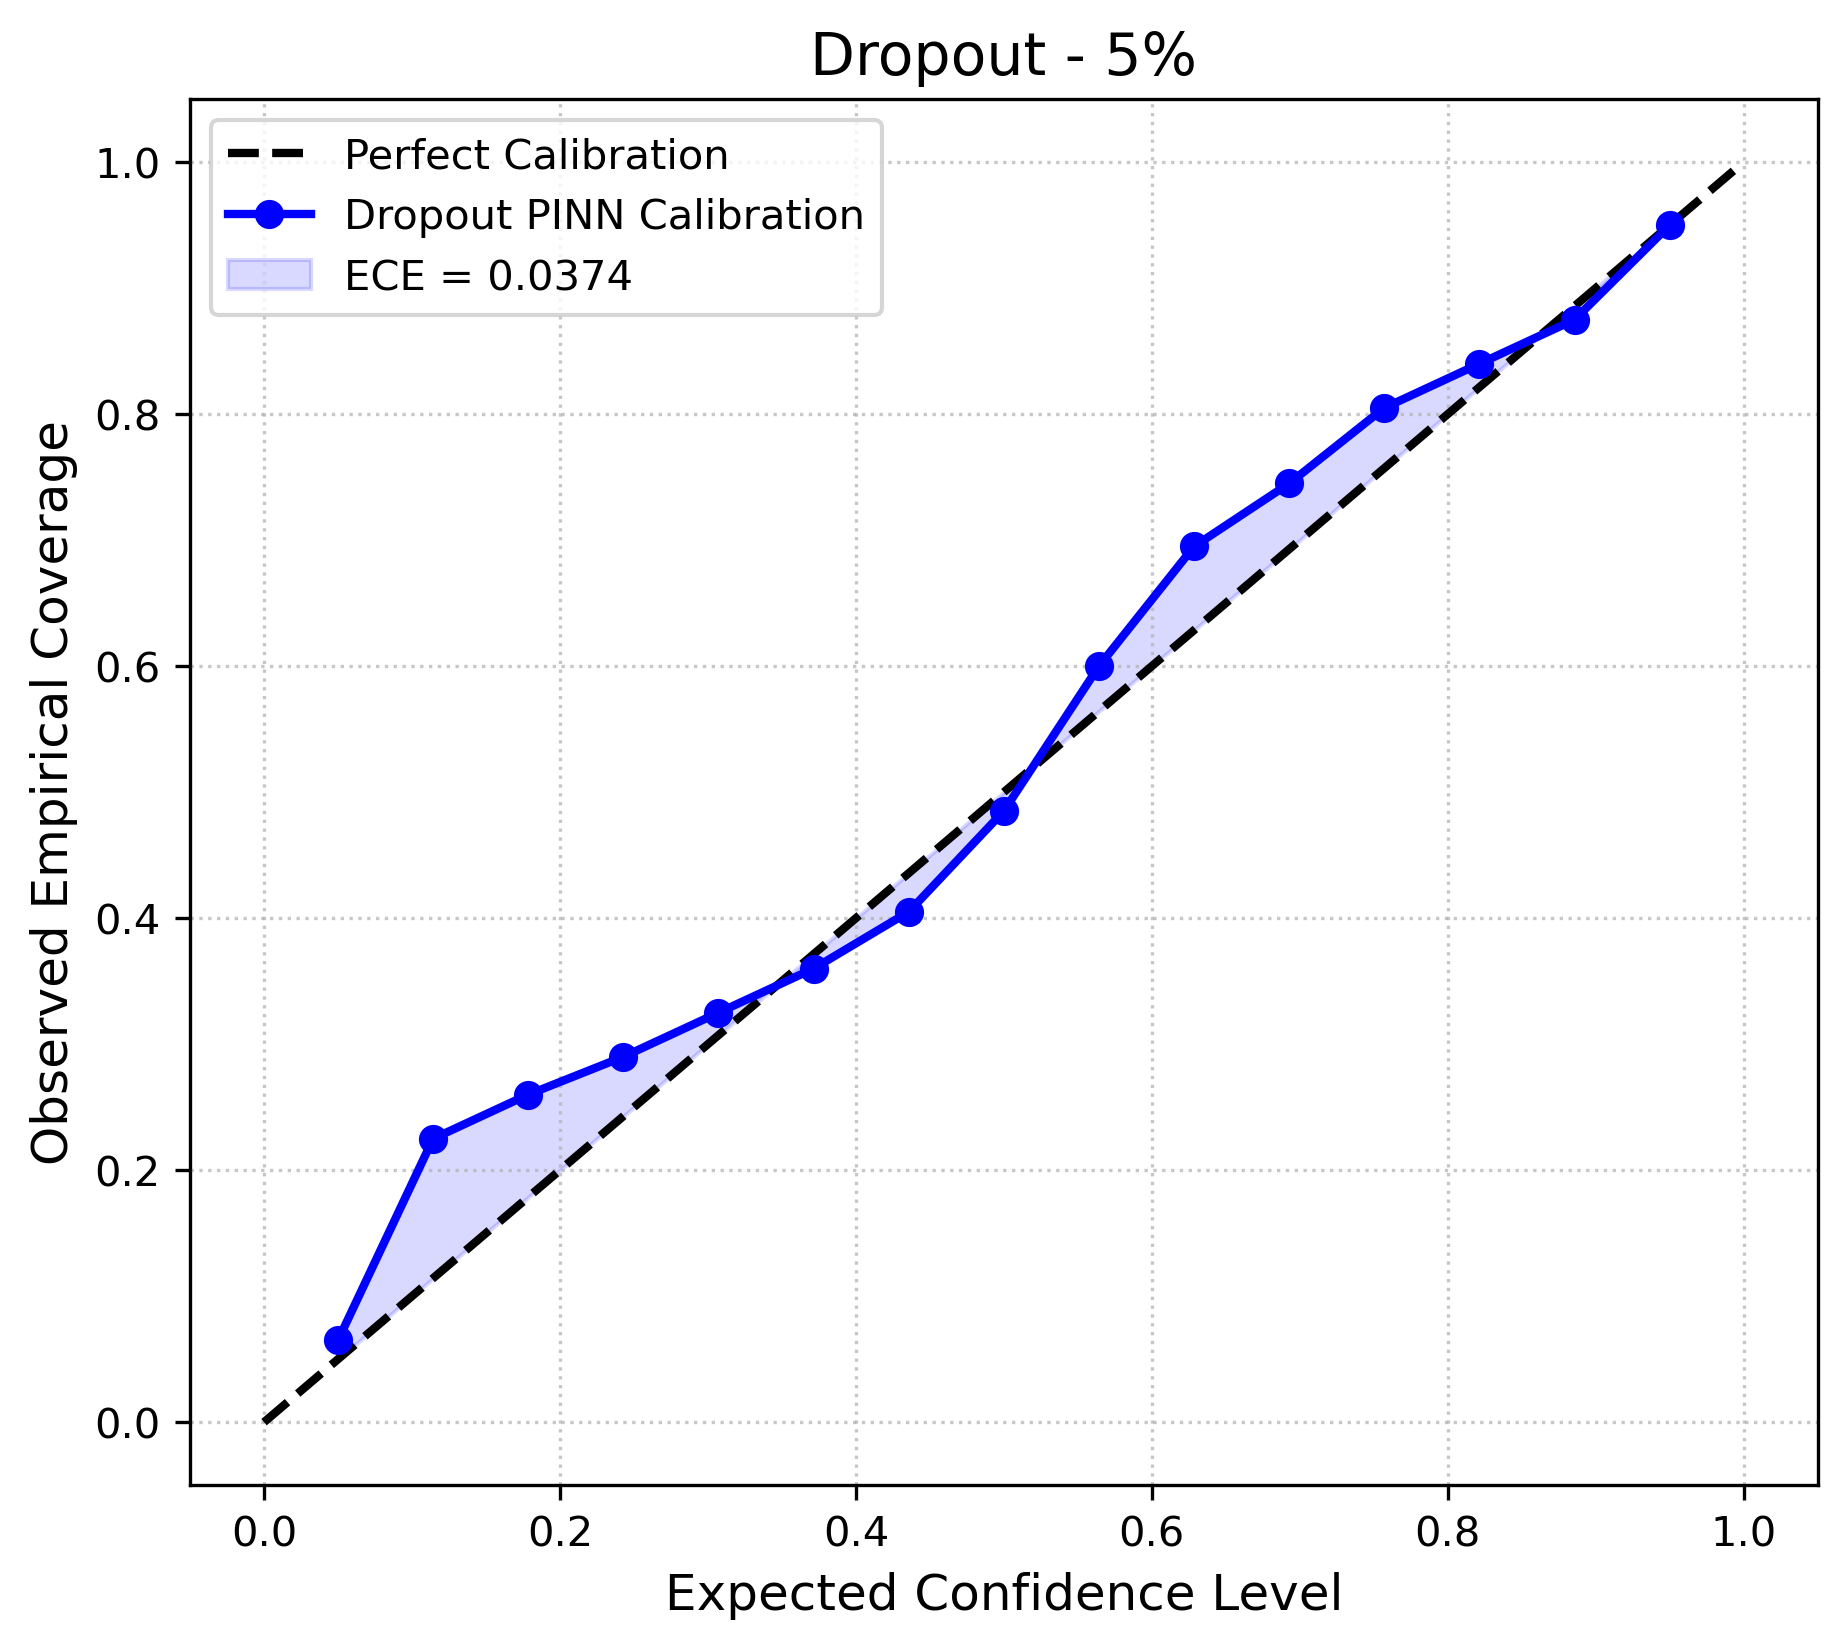
\includegraphics[width=\linewidth]{Figures/dropout/dropout_reliability_1_5.png} % Replace with your third image file
    \caption{}
    \label{fig:image3}
\end{subfigure}
\caption{ \footnotesize Reliability Diagrams for B-PINN and Dropout-PINN on the 1D Poisson Equation, with $\sigma_f = 0.1$ and $\sigma_b = 0.1$ for (a),(c),(d), and a prior on the noise ($\sigma_b$) for (b) }
\end{figure}


\begin{table}[h]
\centering
\footnotesize
\begin{tabular}{|c|c|c|c|c|c|}
\hline
 & B-PINN & B-PINN (unknown noise)  & PINN & Dropout 5\% & Dropout 1\%   \\
\hline
Relative $L^2$ norm & 0.2220  & 0.2492  &   0.0324 & 0.4341 & 0.3059  \\
\hline
PICP( \%) & 100 & 100 & - & 86.00 & 95.50 \\
\hline
MPIW & 0.6389 & 0.3887 & - & 0.7398 & 0.4462 \\
\hline
NLL & -0.6452 & -0.8415  & - & -0.0357 & -0.3265 \\
\hline
ECE &  0.0640 & 0.2432 & - & 0.0367 & 0.1950\\
\hline
\end{tabular}
\caption{ \footnotesize Metrics for the 1D poisson equation forward problem with measurement noise 0.01}
\label{tab:5x5}
\end{table}

\begin{figure}[h]
\centering
% Première ligne : PINN et BPINN
\begin{subfigure}{0.3\textwidth}
    \centering
    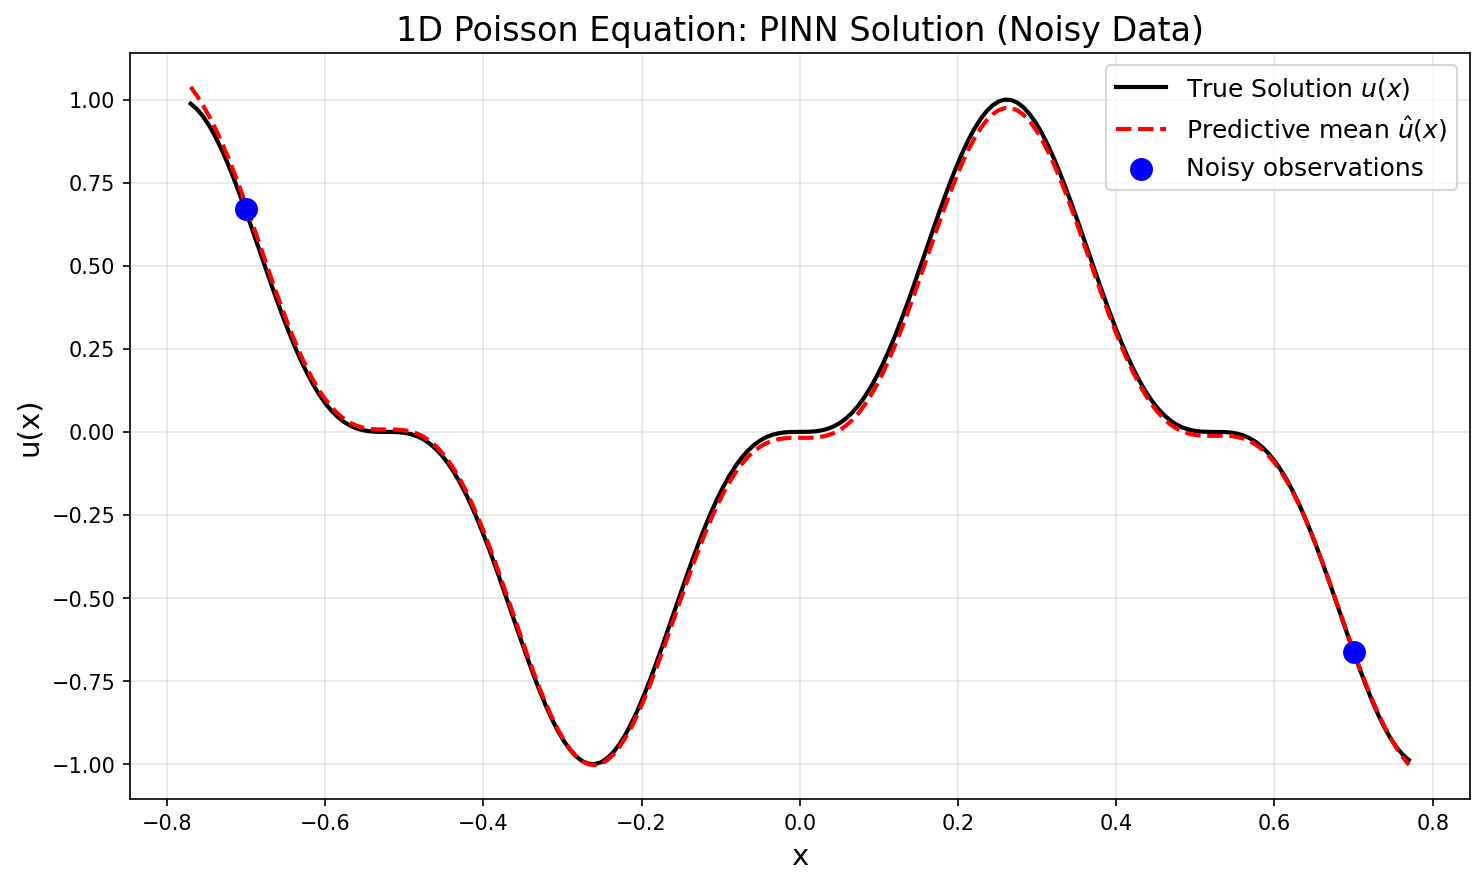
\includegraphics[width=\linewidth]{Figures/1D poisson sigma = 0.01/PINN.png}
    \caption{}
    \label{fig:image2}
\end{subfigure}\hfill
\begin{subfigure}{0.3\textwidth}
    \centering
    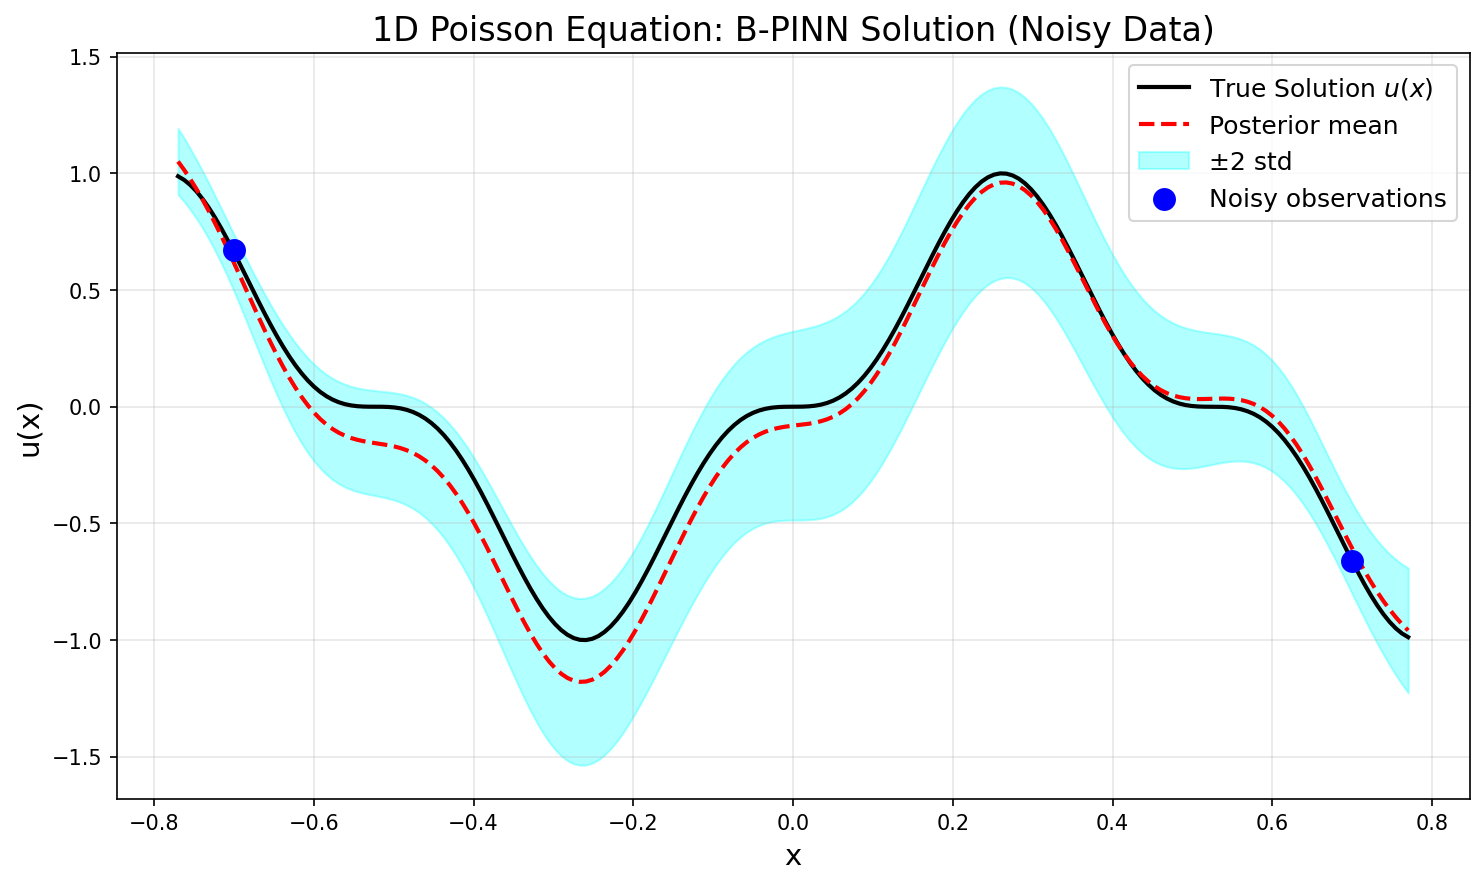
\includegraphics[width=\linewidth]{Figures/1D poisson sigma = 0.01/BPINN.png}
    \caption{}
    \label{fig:image1}
\end{subfigure}
\begin{subfigure}{0.3\textwidth}
    \centering
    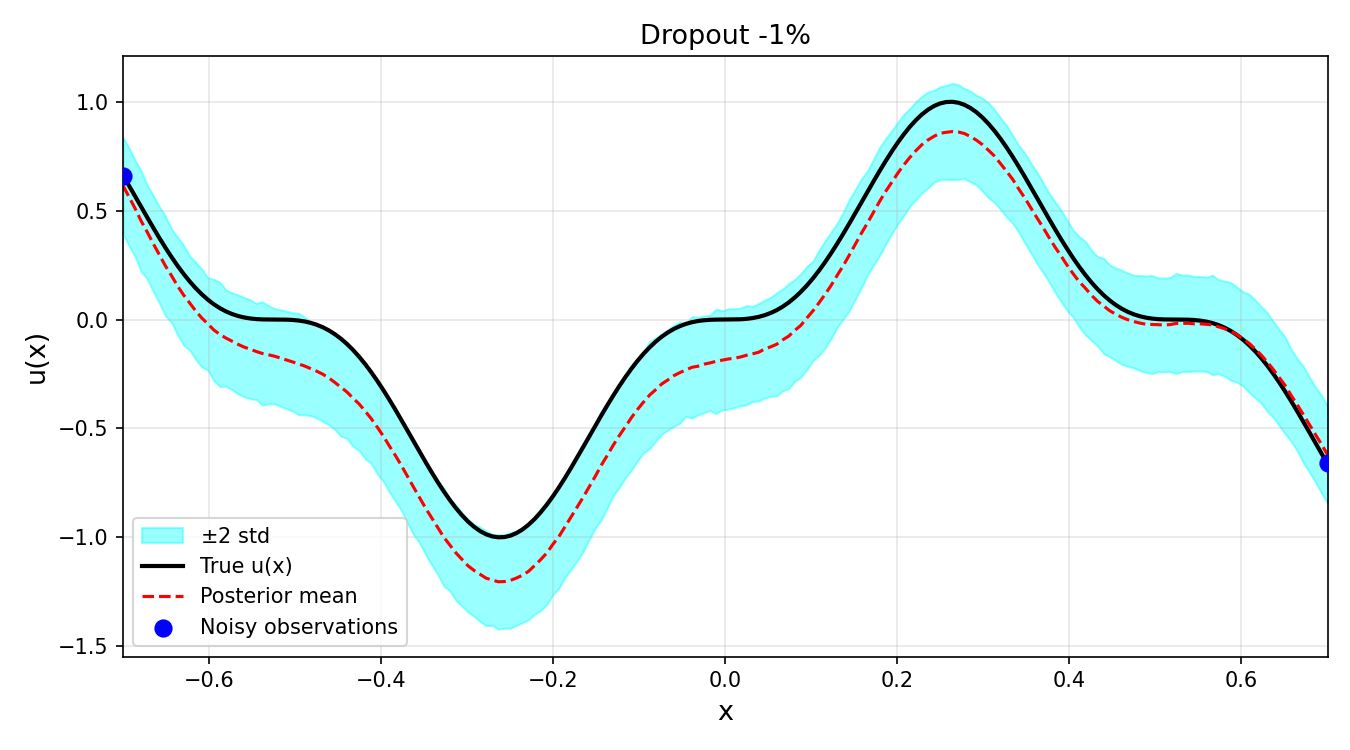
\includegraphics[width=\linewidth]{Figures/dropout/dropout_1_01.png}
    \caption{}
    \label{fig:drop}
\end{subfigure}
\hfill\begin{subfigure}{0.3\textwidth}
    \centering
    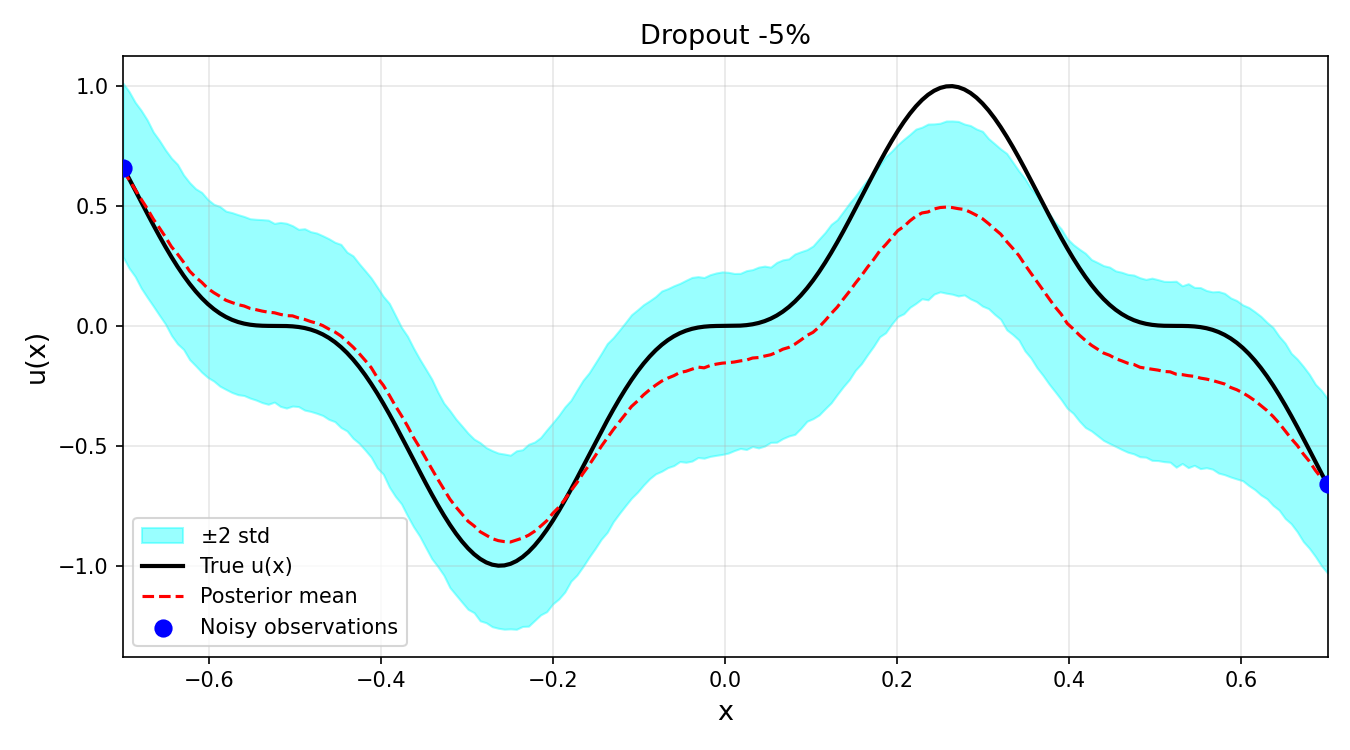
\includegraphics[width=\linewidth]{Figures/dropout/dropout_5_01.png}
    \caption{}
    \label{fig:drop}
\end{subfigure}
\begin{subfigure}{0.3\textwidth}
    \centering
    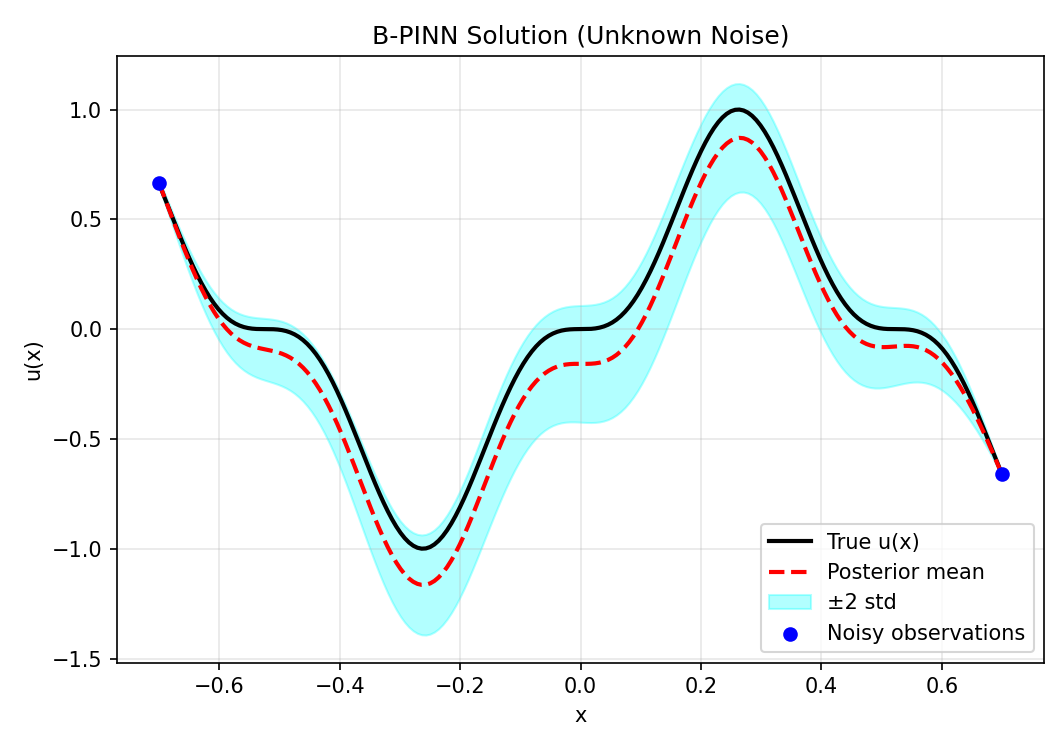
\includegraphics[width=\linewidth]{Figures/1D poisson sigma = 0.01/HBPINN_modif.png}
    \caption{}
    \label{fig:image3}
\end{subfigure}
\caption{ \footnotesize 1D linear Poisson equation- forward problem: predicted u from different methods with noise scale $\epsilon_f \sim \mathcal{N}(0,0.01^2)$ and $\epsilon_b \sim \mathcal{N}(0,0.01^2)$. (e) B-PINN with prior on $\sigma_f$.}
\label{fig:noise01}
\end{figure}





\begin{figure}[h]
\centering
\begin{subfigure}{0.24\textwidth}
    \centering
    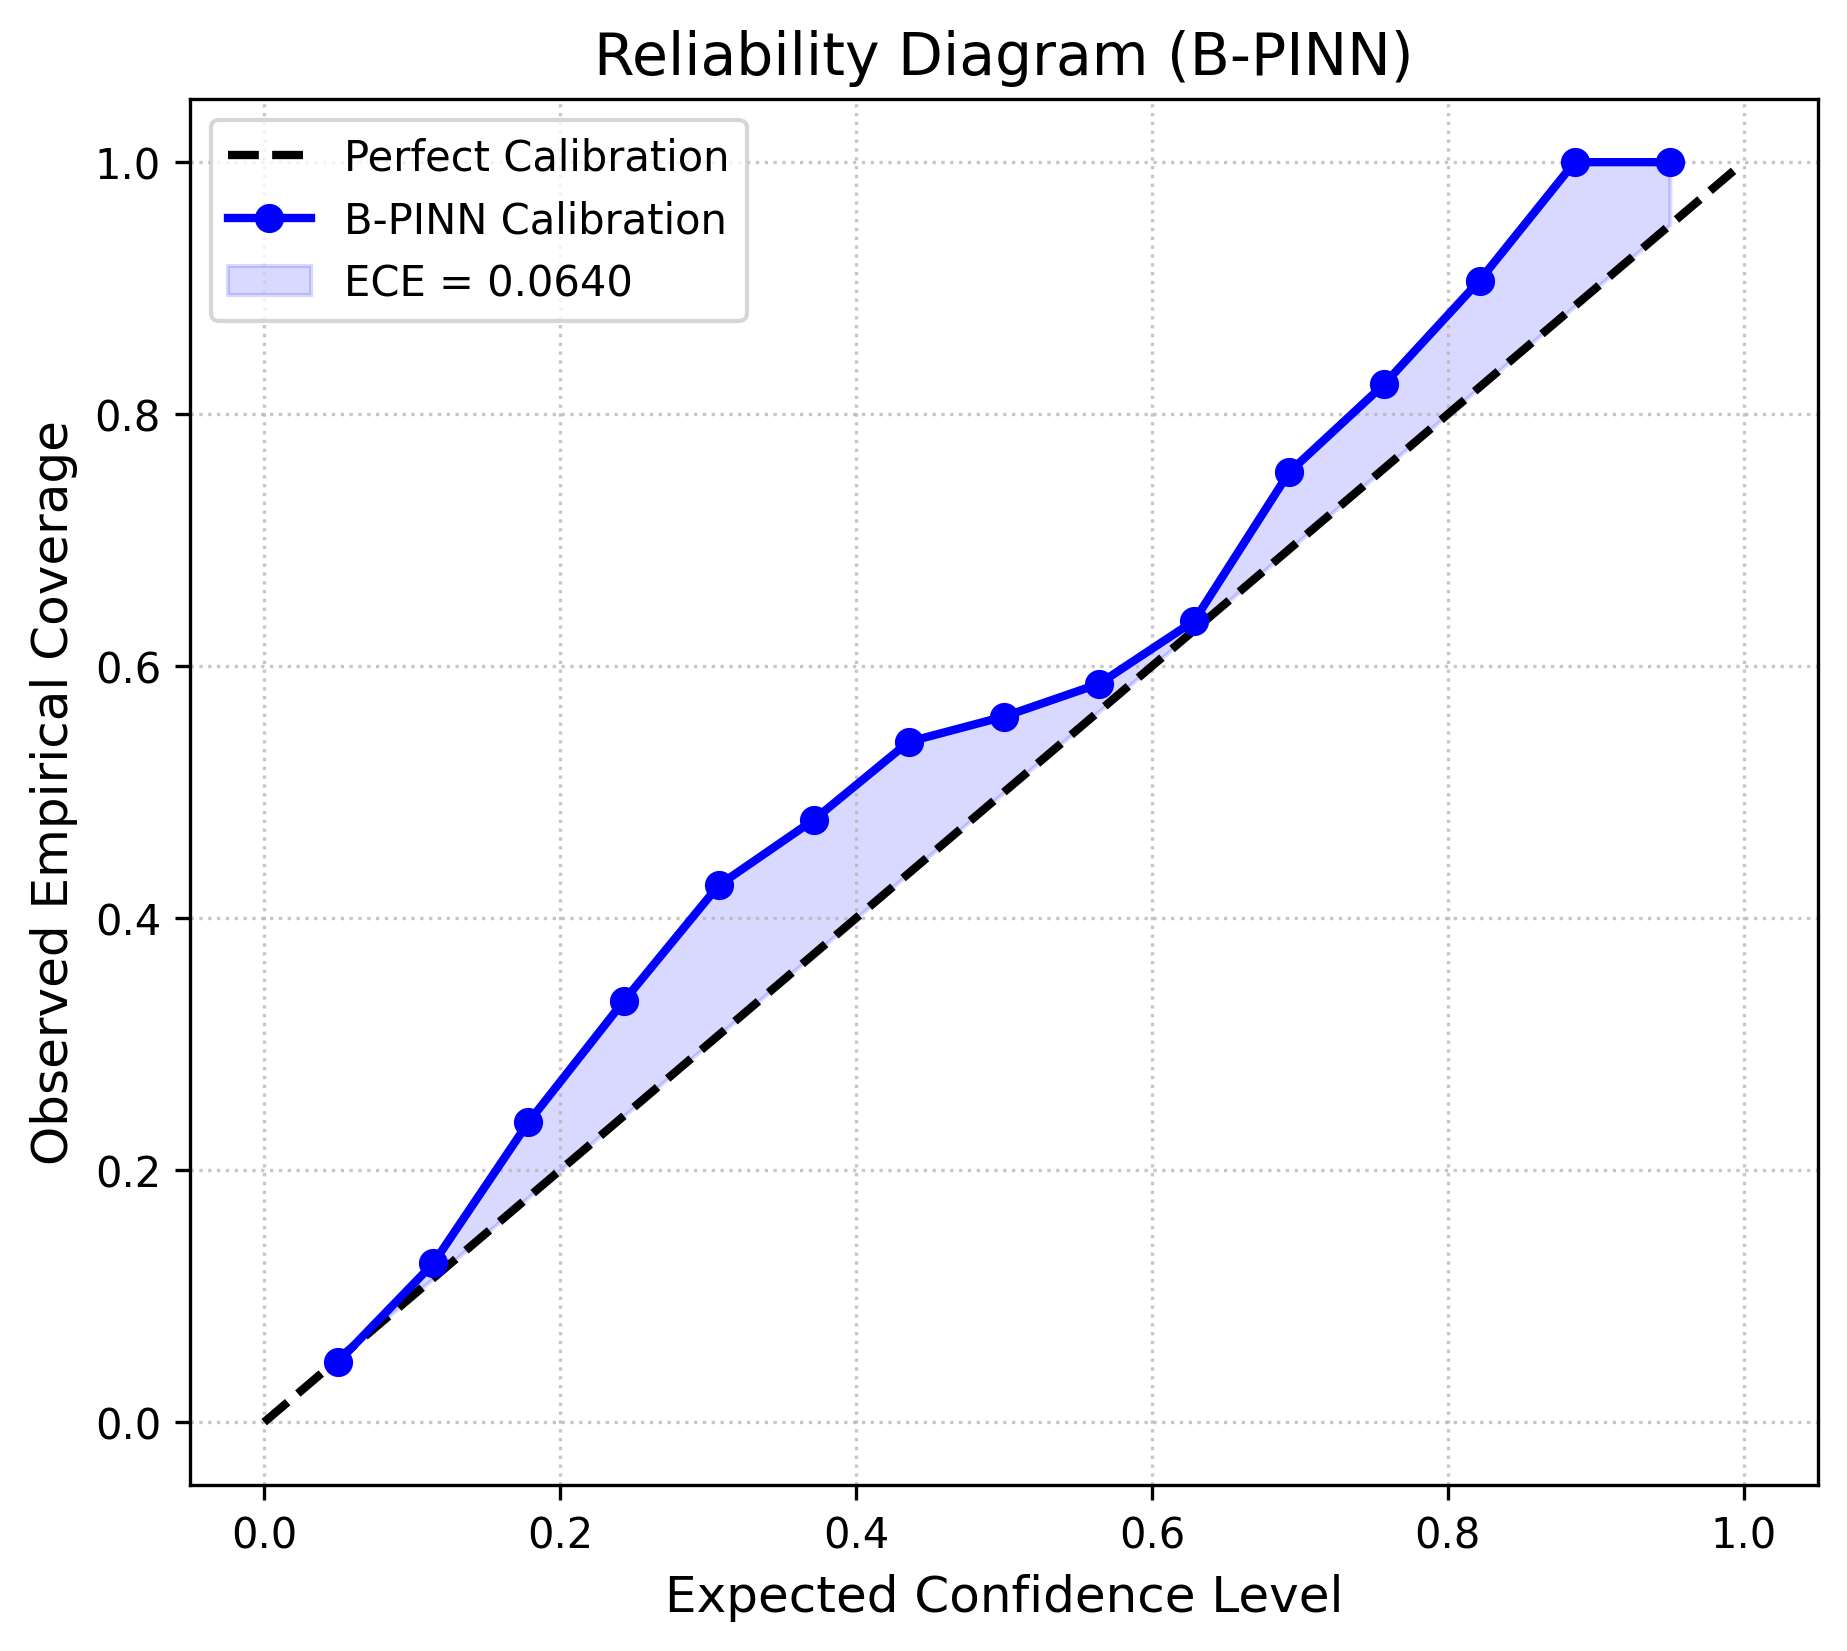
\includegraphics[width=\linewidth]{Figures/1D poisson sigma = 0.01/BPINN_reliability.png}
    \caption{}
    \label{fig:image1}
\end{subfigure}
\begin{subfigure}{0.24\textwidth}
    \centering
    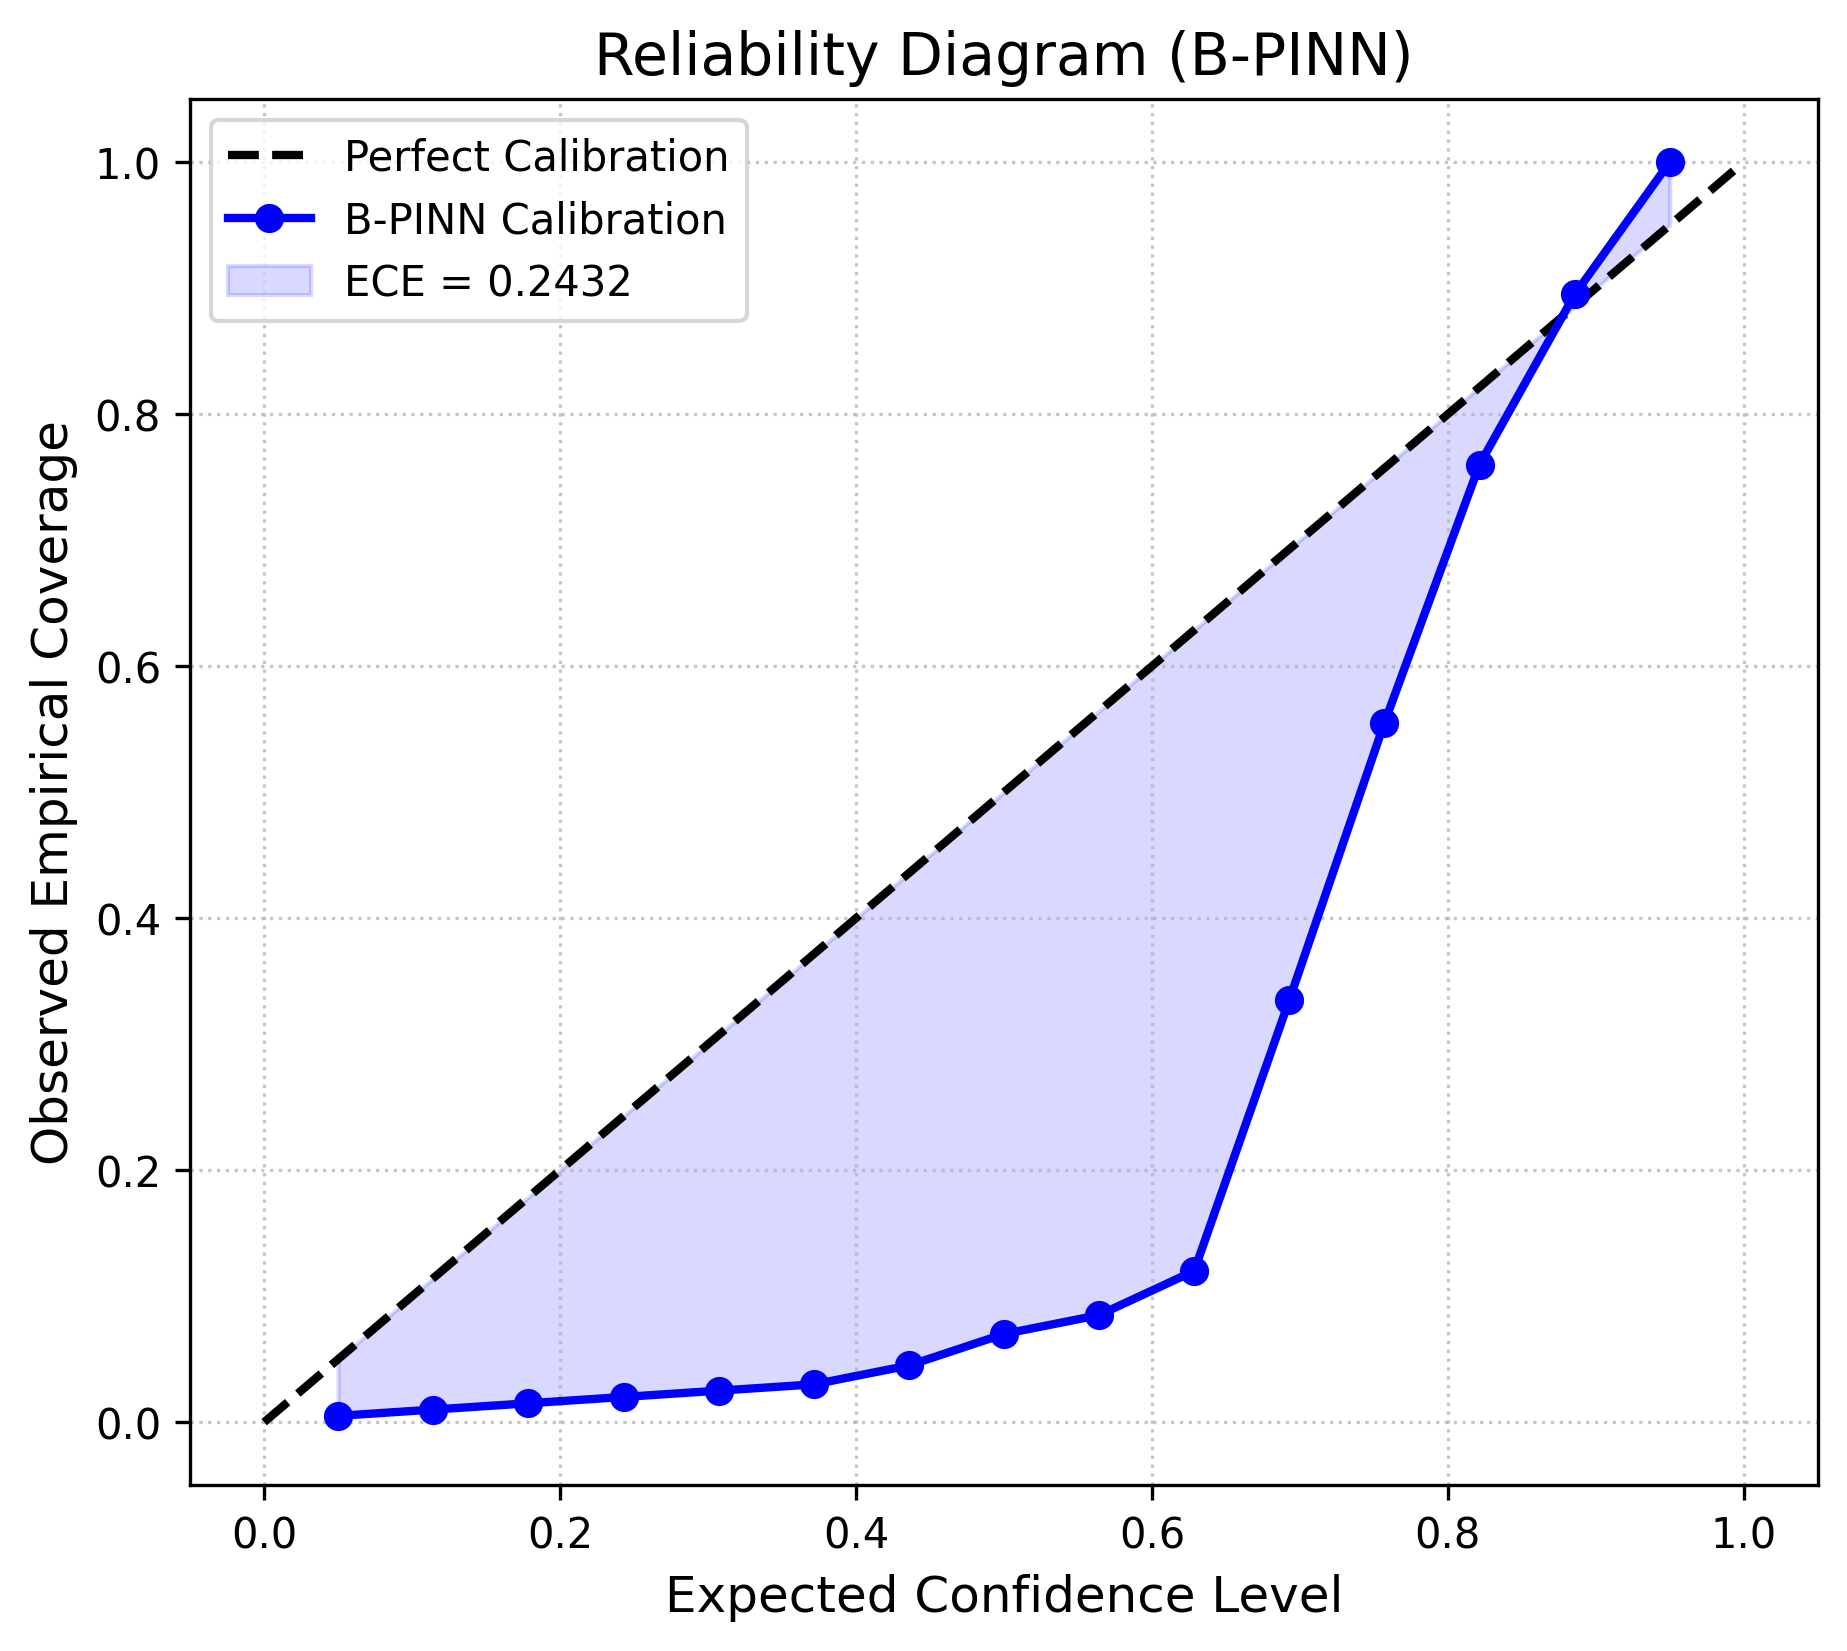
\includegraphics[width=\linewidth]{Figures/1D poisson sigma = 0.01/HBPINN_reliability.png}
    \caption{}
    \label{fig:image2}
\end{subfigure}
\begin{subfigure}{0.24\textwidth} 
    \centering
    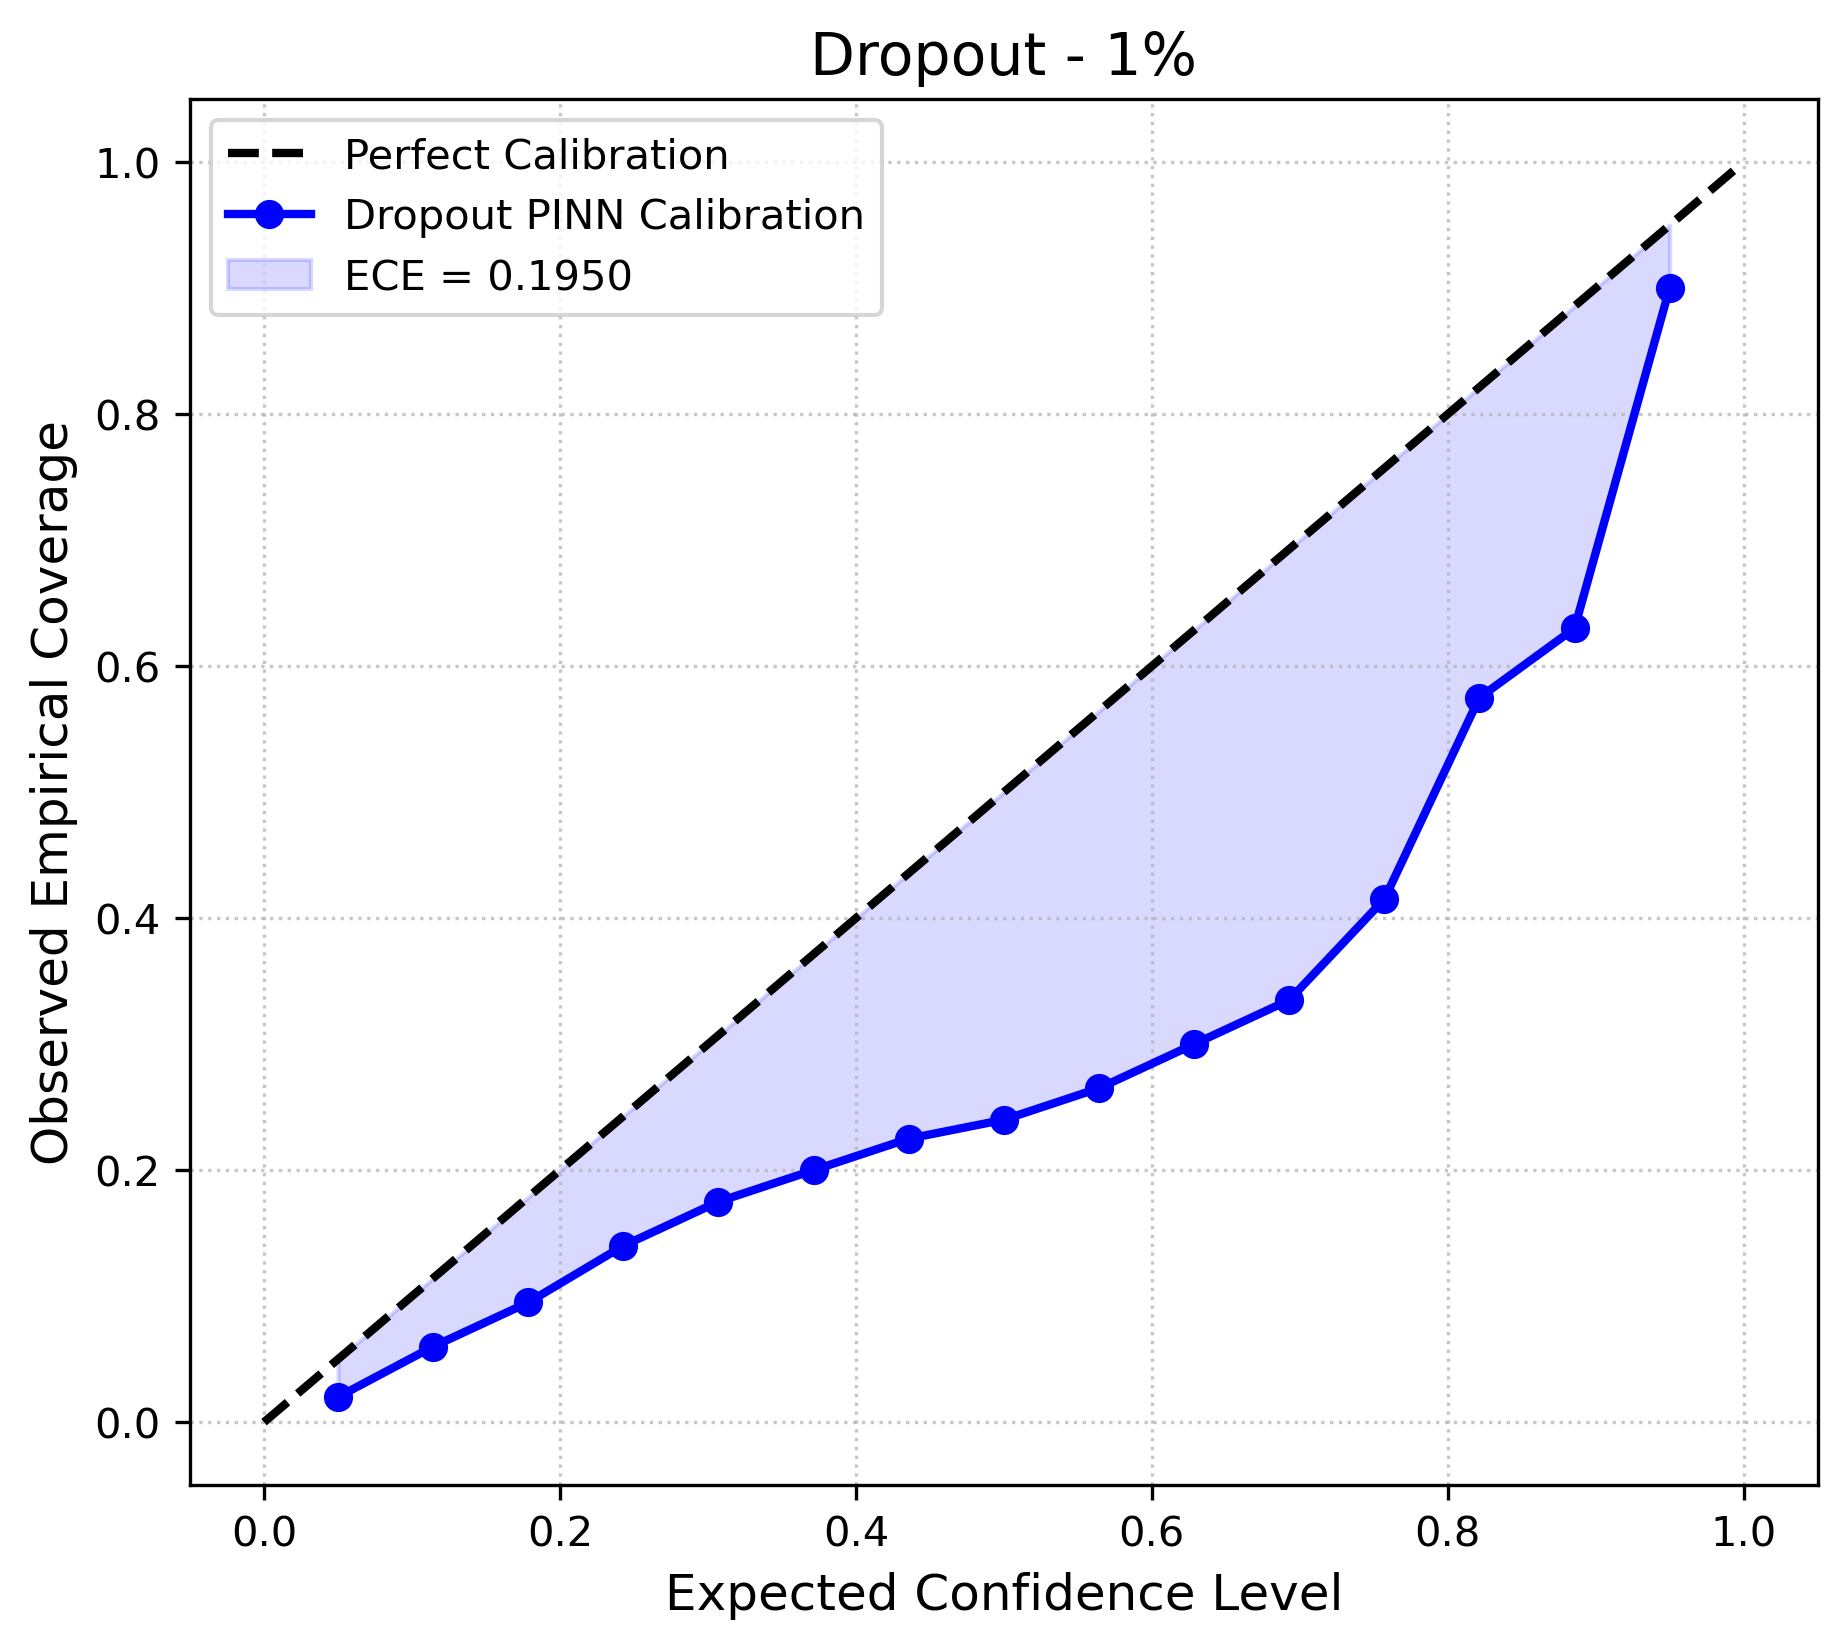
\includegraphics[width=\linewidth]{Figures/dropout/dropout_reliability_1_01.png} % Replace with your third image file
    \caption{}
    \label{fig:image3}
\end{subfigure}
\begin{subfigure}{0.24\textwidth} 
    \centering
    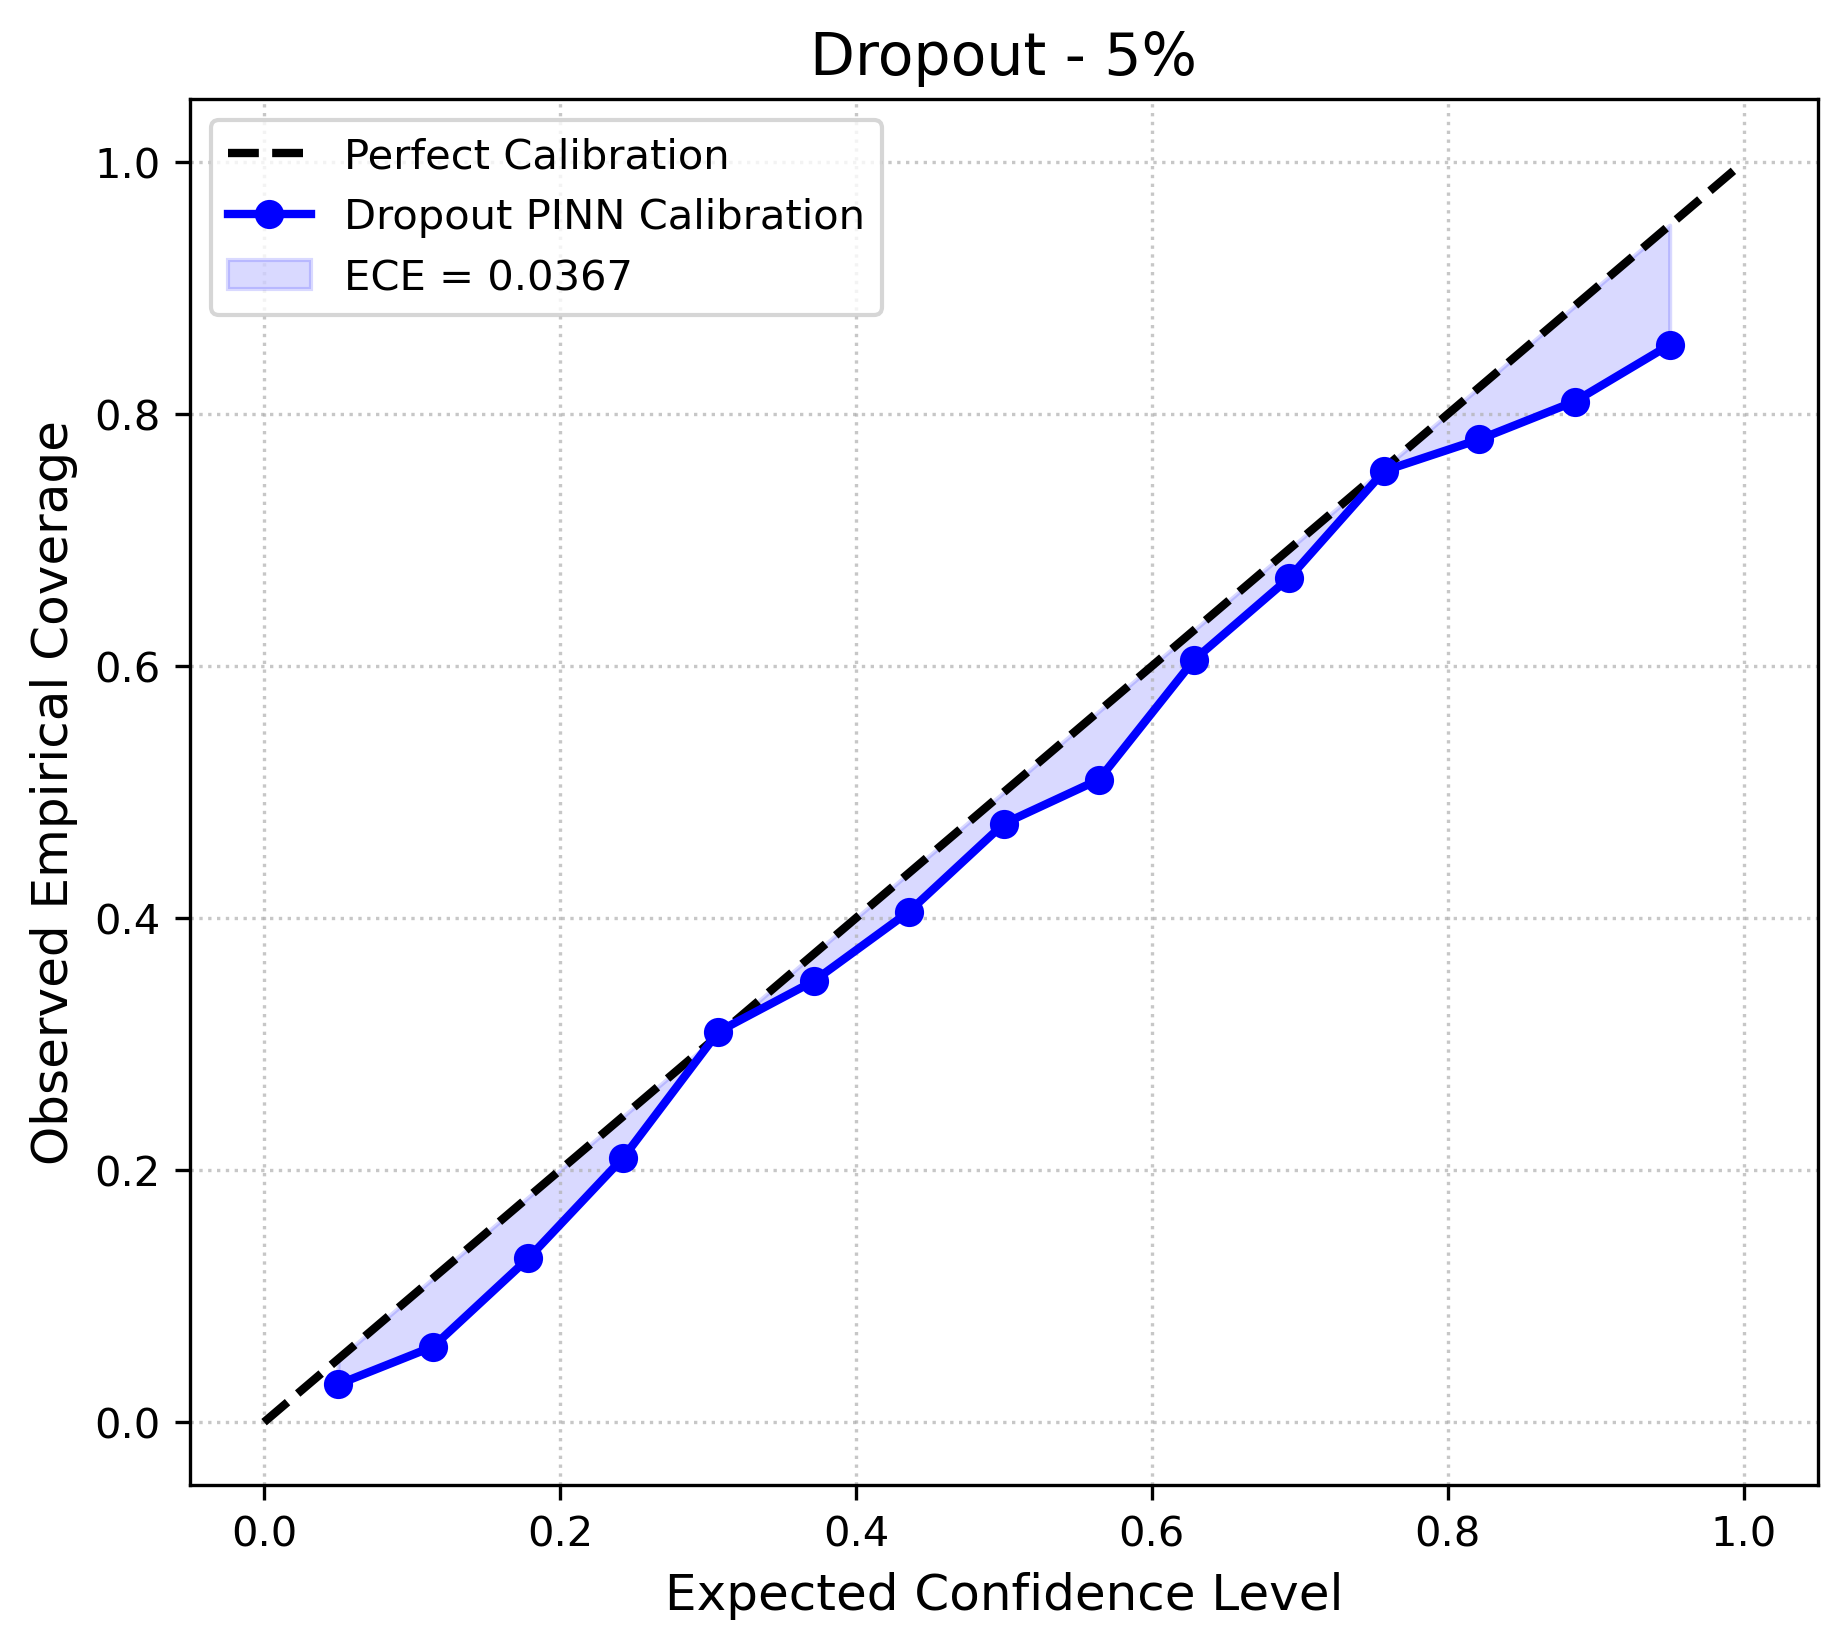
\includegraphics[width=\linewidth]{Figures/dropout/dropout_reliability_5_01.png} % Replace with your third image file
    \caption{}
    \label{fig:image3}
\end{subfigure}
\caption{\footnotesize Reliability Diagrams for B-PINN and Dropout-PINN on the 1D Poisson Equation, with $\sigma_f = 0.01$ and $\sigma_b = 0.01$ for (a),(c),(d), and a prior on the noise ($\sigma_b$) for (b) }
\end{figure}


\paragraph{High noise setting: the B-PINN beats the PINN.}  Under high noise conditions ($\sigma=0.1$), the standard PINN performs poorly, resulting in a high relative L2 error (0.4338). Because it relies on deterministic gradient descent, it tends to overfit the noisy sensor data, distorting the underlying wave shape. In contrast, the B-PINN reduces this overfitting, dropping the L2 error to 0.2952. By averaging across a probability distribution of network weights, the B-PINN smooths out the high-frequency noise and treats the physical equations as flexible guidelines rather than strict rules. This confirms the result of the paper.


\paragraph{Low noise setting: the low noise identifiability trap.} In this setting, the B-PINN with unknown noise fails to find the true value of the noise and largely inflates it. Nevertheless, despite failing to accurately pinpoint the 0.01 noise scale, it still yields a highly respectable predictive mean (L2 = 0.2492) and perfectly bounds the true solution (PICP = 100\%). It proves that even when a Bayesian model misidentifies the source of the error, the dynamic noise parameter acts as a robust safety valve that prevents the HMC sampler from diverging.

\paragraph{High noise setting: the B-PINN with a prior beats the vanilla B-PINN.}
The B-PINN with a prior on the noise achieved the best overall performance in that regime. This seems counter-intuitive as providing a B-PINN with the exact, true noise variance should yield the optimal fit, we provide a possible explanation. This could occur  because $\sigma_f$ acts as an adaptive weighting mechanism between the data likelihood and the physical constraints.  When fixed to the true noise level, the network may still retain enough flexibility to overfit the specific noise realization, thereby corrupting the physics. By allowing $\sigma_f$ to be learned dynamically, the model can artificially inflate the inferred noise scale when data points heavily contradict the physics residual. This inflation down-weights the data loss penalty, granting the model the mathematical freedom to ignore the chaotic data and prioritize a smooth, physically consistent solution.


\paragraph{Low noise setting: the PINN outperforms B-PINNS.}  In the low noise setting ($\sigma = 0.01$), the PINN vastly outperforms the Bayesian models here, achieving an L2 error of 0.0324. When the data is clean, a standard optimizer can easily find the exact global minimum of the physics loss. 
B-PINNs (L2 = 0.2220), however, are designed to explore a distribution rather than lock onto a single point. In low-noise scenarios, the target distribution becomes incredibly narrow and steep. Because the HMC sampler constantly moves around this narrow target to capture uncertainty—rather than resting exactly at its center, its averaged prediction slightly misses the exact ground truth, resulting in a higher error than the deterministic PINN.

\paragraph{The failure of dropout as a Bayesian Proxy.} Dropout's uncertainty bands are dictated by the dropout rate rather than the actual physical noise. At high noise ($\sigma=0.1$), Dropout 1\% yields a catastrophic PICP of only 54.0\%, meaning nearly half the true solution falls outside its confidence bands. The reliability diagram (Figure 2c) makes this failure vivid: the empirical coverage curve lies far below the diagonal across all confidence levels, confirming systematic underestimation of uncertainty. The ECE further highlights this. A perfectly calibrated model has an ECE near 0. At high noise, Dropout 1\% has an ECE of 0.3090 (highly uncalibrated). While Dropout 5\% achieves a better PICP (95.5\%), it does so simply by inflating its bands massively (MIPW of 0.7864), acting as a blunt instrument rather than a precise mathematical measure of variance. Comparing the two noise regime reveals that the MPIW  is dictated almost entirely by the chosen dropout rate rather than the data's noise. Dropout 1\% maintains a narrow band  regardless of the regime. While this narrow band accidentally yields excellent coverage when the noise is low (PICP = 95.50\%), it fails catastrophically when the noise increases (PICP = 54.00\%). 

\paragraph{The impact of the prior on the noise on the uncertainty.}
Under the high-noise setting ($\sigma = 0.1$), the B-PINN with a prior on the noise generates a slightly wider, more conservative uncertainty band compared to the standard B-PINN (MPIW of 0.7137 vs. 0.6465). This adaptive widening allows it to achieve perfect coverage of the true solution as the dynamically learned noise parameter acts as a safety valve that down-weights chaotic data in favor of physical constraints. Conversely, in the low-noise regime ($\sigma = 0.01$), the it struggles to accurately pinpoint the minute noise scale and artificially inflates it. Interestingly, despite this misidentification, it produces a significantly tighter predictive interval than the standard B-PINN (MPIW of 0.3887 vs. 0.6389) while still maintaining 100\% coverage.
A possible explanation is that the standard B-PINN's wider uncertainty band in the low-noise setting is actually stemming from numerical error from the HMC that is struggling to sample a space that is too sharp ( the low noise means the target distribution is very sharp), hence the HBPINN is avoiding this numerical trap by inflating the noise.

\subsection{Bridging Bayesian PINNs and Gaussian Processes (PI-GP)}
As a second extension, we decided to explore the theoretical properties and ultimate limits of Bayesian PINNs.We investigate their behavior as the neural network architecture scales. Specifically, what is the exact mathematical object that a B-PINN approximates, and how does its practical implementation via HMC differ from this theoretical limit?

\subsubsection{The Infinite-Width Limit: BNNs as NNGPs}

Consider a fully-connected multilayer perceptron mapping inputs $x \in \mathbb{R}^{d_{in}}$ to a scalar output $u_L(x)$, featuring $L$ hidden layers of width $N_l$. The network computes $h^{(l)}(x) = \phi\big(W^{(l)} h^{(l-1)}(x) + b^{(l)}\big)$, where $W^{(l)}_{ij} \sim \mathcal{N}(0, \sigma_w^2 / N_{l-1})$ and $b^{(l)}_i \sim \mathcal{N}(0, \sigma_b^2)$.
By the Central Limit Theorem, as the hidden layer widths $N_l \to \infty$, the pre-activations of each layer converge in distribution to a multivariate Gaussian \cite{Lee2018}. Consequently, the output surrogate function converges entirely to a Gaussian Process:
\begin{equation*}
u(\cdot;\theta) \xrightarrow[N_1, \dots, N_L \to \infty]{\text{Distribution}} \mathcal{GP}\big(0, k_{\text{NNGP}}(\cdot, \cdot)\big)
\end{equation*}
The prior covariance kernel $k_{\text{NNGP}}$ is recursively determined by the network depth, variance priors ($\sigma_w^2, \sigma_b^2$), and the activation function $\phi$:
\begin{equation*}
K^{(0)}(x, x') = \frac{\sigma_w^2}{d_{in}} x \cdot x' + \sigma_b^2 \quad \quad K^{(l)}(x, x') = \sigma_w^2 \mathbb{E}_{(z, z') \sim \mathcal{N}(0, \Sigma^{(l-1)})} \Big[ \phi(z) \phi(z') \Big] + \sigma_b^2
\end{equation*}
where: 
\begin{equation*}
\quad \Sigma^{(l-1)} = \begin{pmatrix} K^{(l-1)}(x, x) & K^{(l-1)}(x, x') \\ K^{(l-1)}(x', x) & K^{(l-1)}(x', x') \end{pmatrix}
\end{equation*}

\subsubsection{Gaussian Processes under Linear Differential Operators}
Having analytically established that the BNN prior is $u \sim \mathcal{GP}\big(0, k_{\text{NNGP}}(x, x')\big)$, we must apply the PDE and boundary constraints. If the differential operator $\mathcal{L}_x$ is linear, its application to the Gaussian Process $u(x)$ yields another Gaussian Process. 
Leveraging the linearity of expectation, the spatial differential operators commute outside the covariance expectation bracket, yielding analytically exact cross-covariances linking the state evaluation to the physical derivative evaluation:
\begin{equation}
\text{Cov}\big(u(x), \mathcal{L}_{x'} u(x')\big) = \mathcal{L}_{x'} k(x, x'), \qquad \text{Cov}\big(\mathcal{L}_x u(x), \mathcal{L}_{x'} u(x')\big) = \mathcal{L}_x \mathcal{L}_{x'} k(x, x')
\end{equation}

\subsubsection{The Exact Physics-Informed GP (PI-GP)}
We construct an overarching block observation vector $Y = [\bar u, \bar f, \bar b]^T = \mathcal{A} u + \epsilon$, where $\epsilon \sim \mathcal{N}(0, \Sigma_{\text{noise}})$ and $\Sigma_{\text{noise}} = \text{blockdiag}(\sigma_u^2 I_{N_u}, \sigma_f^2 I_{N_f}, \sigma_b^2 I_{N_b})$. 
These observations follow a vast joint multivariate Normal distribution governed strictly by the structural derivatives of the kernel. We explicitly construct the dense generalized block covariance $\mathbf{K}$:
\begin{equation}
\mathbf{K} = \begin{bmatrix}
k(X_u, X_u) & \mathcal{L}_{x'}k(X_u, X_f) & \mathcal{B}_{x'}k(X_u, X_b) \\
\mathcal{L}_x k(X_f, X_u) & \mathcal{L}_x \mathcal{L}_{x'} k(X_f, X_f) & \mathcal{L}_x \mathcal{B}_{x'} k(X_f, X_b) \\
\mathcal{B}_x k(X_b, X_u) & \mathcal{B}_x \mathcal{L}_{x'} k(X_b, X_f) & \mathcal{B}_x \mathcal{B}_{x'} k(X_b, X_b)
\end{bmatrix}
\end{equation}
For any arbitrary spatial query point $x^*$, the cross-covariance is $\mathbf{k}_{*} = \begin{bmatrix} k(x^*, X_u) & \mathcal{L}_{x'}k(x^*, X_f) & \mathcal{B}_{x'}k(x^*, X_b) \end{bmatrix}$. The infinite-width, physics-informed posterior probability field evaluated at $x^*$ is analytically given by the closed-form standard GP regression:
\begin{equation}
\mu(x^*) = \mathbf{k}_{*} (\mathbf{K} + \Sigma_{\text{noise}})^{-1} Y, \qquad \Sigma(x^*) = k(x^*, x^*) - \mathbf{k}_{*} (\mathbf{K} + \Sigma_{\text{noise}})^{-1} \mathbf{k}_{*}^T \label{eq:pigp_posterior}
\end{equation}
This formulation provides mathematically convex, resolution-free analytical posteriors, bypassing the need for computationally unstable HMC sampling.

\subsubsection{Empirical Evaluation: The Expressivity vs. Adaptivity Trade-off}
While the infinite-width limit provides a mathematically rigorous formulation, empirical evaluation reveals a fundamental limitation of the NNGP in capturing highly oscillatory physical dynamics. We benchmarked the exact PI-GP formulation on the 1D Poisson equation where the true solution is $u(x) = \sin^3(6x)$. We tested two observational noise scales: $\sigma = 0.01$ and $\sigma = 0.1$.

\begin{figure}[h]
    \centering
    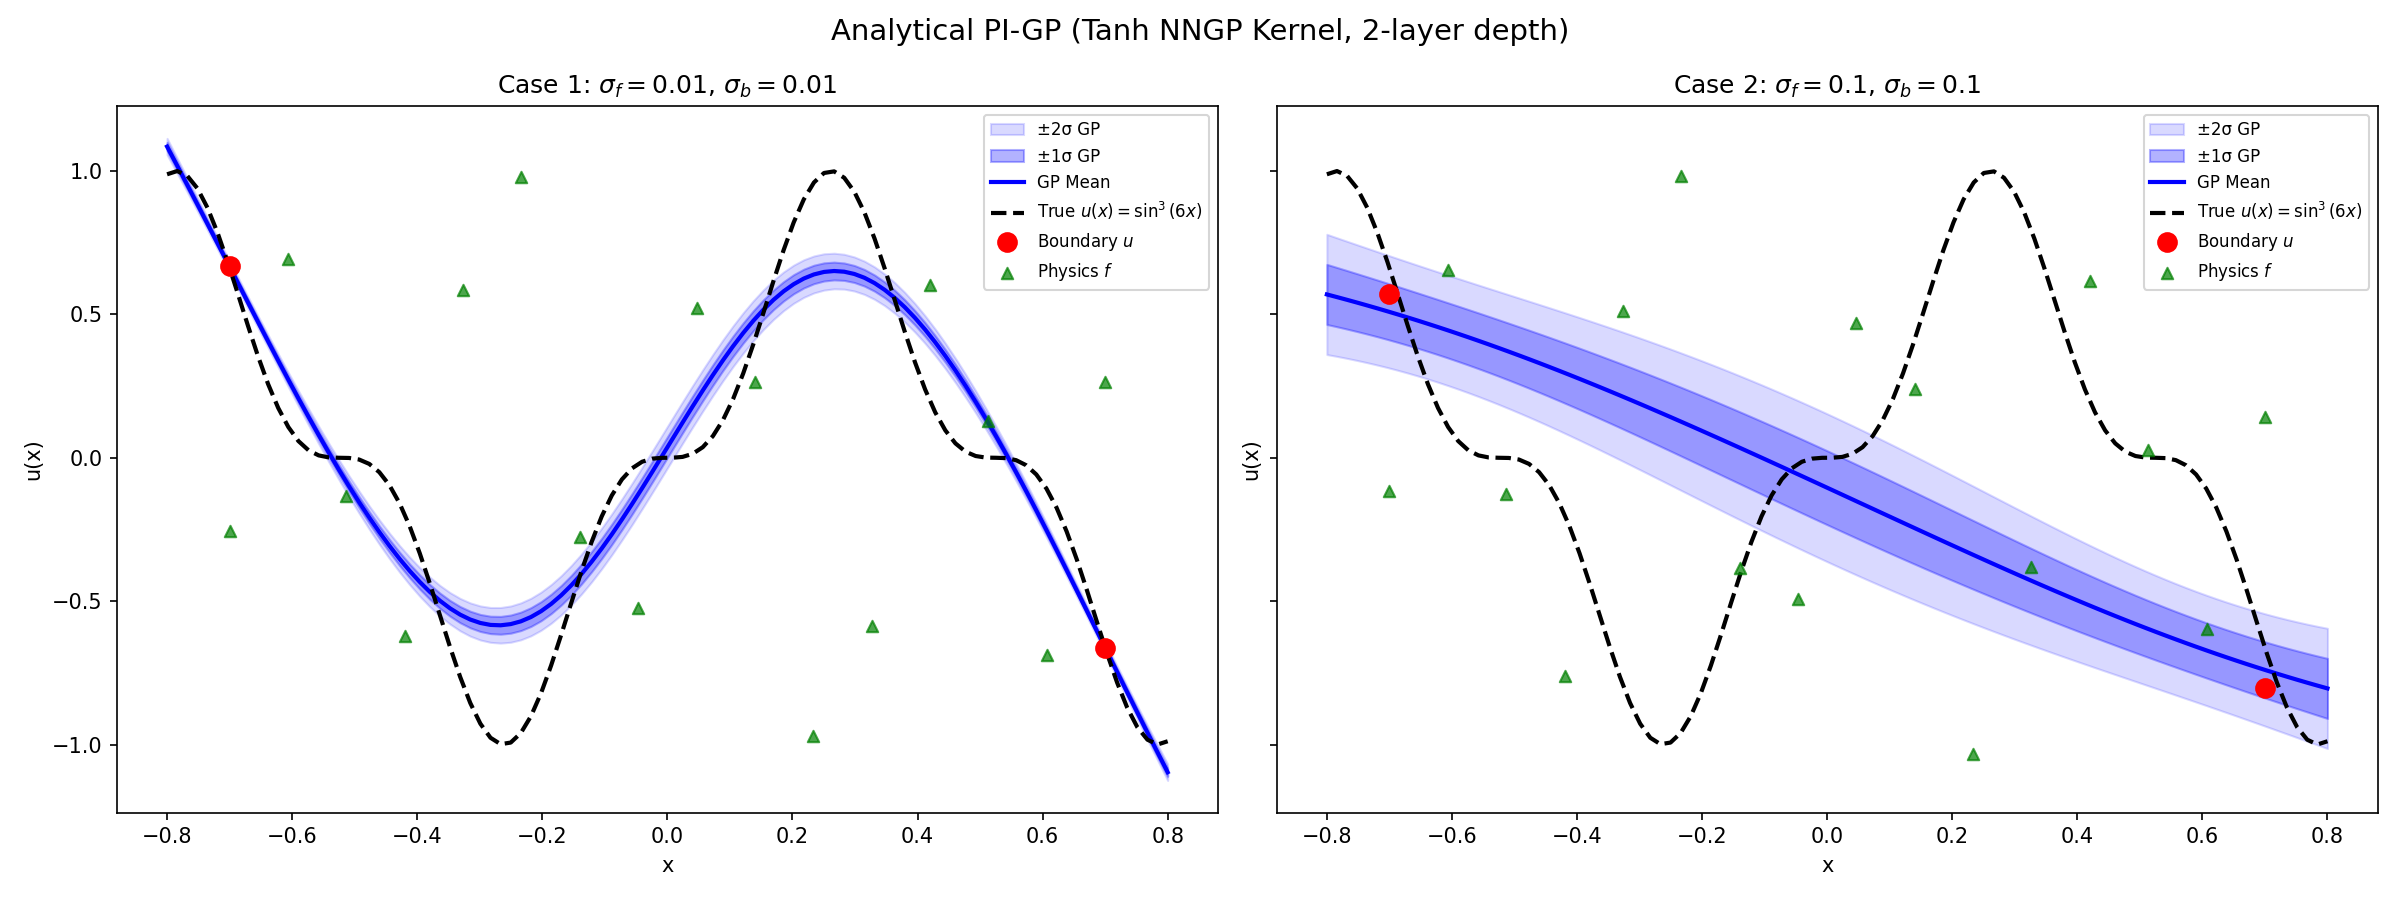
\includegraphics[width=0.7\textwidth]{Figures/GP/test_gp_result.png}
    \caption{\footnotesize Comparison of the exact PI-GP posterior mean and 2-sigma confidence interval against the true solution for the 1D Poisson equation with $u(x) = \sin^3(6x)$. (a) Low noise ($\sigma = 0.01$). (b) High noise ($\sigma = 0.1$).}
    \label{fig:gp_comparison}
\end{figure}

\paragraph{The Curse of the Stationary Kernel and "Lazy Learning":}
As shown in Figure \ref{fig:gp_comparison}, the exact PI-GP struggles to fit the target dynamics, and fails catastrophically when measurement noise increases. Taking the width $N \to \infty$ with i.i.d. Gaussian initializations invokes the Central Limit Theorem, which forces the network into the "lazy training" or Neural Tangent Kernel (NTK) regime. In this limit, the network's feature representations are strictly frozen. The resulting covariance function $k_{\text{NNGP}}(x, x')$ behaves as a rigid, stationary kernel that enforces a global length scale across the entire spatial domain, manifesting as severe \emph{spectral bias}. It is mathematically incapable of being highly oscillatory in one region while remaining smooth in another.

\paragraph{Noise-Induced Prior Dominance:}
This rigidity explains the linear collapse observed at higher noise scales. In the predictive posterior equation (Eq. \ref{eq:pigp_posterior}), the noise matrix $\Sigma_{\text{noise}}$ acts as Tikhonov regularization. When $\sigma = 0.1$, $\Sigma_{\text{noise}}$ scales up dramatically, dominating the physics-physics block covariance $\mathcal{L}_x \mathcal{L}_{x'} k(X_f, X_f)$ inside the matrix inversion. The PI-GP effectively determines that the interior collocation points $X_f$ are too noisy to trust. Stripped of reliable interior data and unable to warp its frozen feature space to isolate the high-frequency sine wave from the noise, the PI-GP falls back entirely on its zero-mean prior, anchoring only to the boundaries and over-smoothing the physics into a linear interpolation.

\paragraph{Representation Learning in Finite B-PINNs:}
In contrast, finite-width B-PINNs (e.g., $N=50$) successfully regress this exact $\sin^3(6x)$ target even at the high $\sigma = 0.1$ noise scale. Finite networks do not fully trigger the Central Limit Theorem collapse, allowing them to perform active \emph{representation learning}. Furthermore, during HMC progression, the massive scale of the data likelihood penalty ($1/\sigma^2$) forces the parameters into an ultra-low norm regime, effectively abandoning the strict Gaussian prior that governs the PI-GP. The parameters actively traverse the posterior landscape, adapting and warping the network's internal non-stationary basis functions to align with the sharp local gradients of the PDE.

Therefore, while the infinite-width PI-GP provides perfect mathematical convexity and correct Gaussian priors for physical derivatives, finite-width B-PINNs remain practically superior for complex, highly oscillatory phenomena due to their unbounded capacity for local feature adaptation.



\section{Conclusion}

This report investigated the efficacy and potential extensions of B-PINNs for solving PDE problems.
We first confirmed the results of \cite{Yang_2021} on the 1D poisson forward problem, demonstrating that B-PINNs indeed out-perform deterministic approaches when large observational noise is present, as well as that dropout is not an efficient alternative to B-PINNs.  By employing HMC sampling to draw from the exact, unnormalized posterior distribution, B-PINNs mitigate the overfitting that plagues standard PINNs trained via gradient descent. Plus, B-PINNs provide predictive uncertainty quantification. Our reliability analysis confirmed that B-PINNs yield well-calibrated confidence intervals, accurately bounding the true underlying physics, whereas heuristic approximations like Monte Carlo Dropout exhibit over-confidence and fail to capture the true posterior variance.

We then explored a first extension, adapting the vanilla B-PINN by adding a prior on the noise instead of giving to the model its true value. This is powerful as in real life scenarios knowing the exact value of the noise is an irrealistic assumption. Furthermore, our result show that this new model performs better than the vanilla B-PINN, even when it fails to predict the true value of the noise. 

Finally, we presented a theoretical bridge between infinite-width B-PINNs and Physics-Informed Gaussian Processe. While the infinite-width limit offers an elegant, closed-form analytical posterior that perfectly enforces linear differential operators, our empirical evaluation uncovered its fundamental weakness: the rigid, stationary nature of the Neural Network Gaussian Process kernel prevents it from capturing highly oscillatory dynamics. We empirically showed that finite-width B-PINNs retain the capacity for feature learning. 

\subsection{Future research}

Future work could explore several promising avenues to extend the capabilities and efficiency of B-PINNs:
\begin{enumerate}
   \item \textbf{Unknown noise in inverse problems:} Although we gave a broad presentation of how to extend the unknown noise model to inverse problems, we have not empirically tested its performance. Validating whether this formulation successfully regularizes inverse problems without sacrificing the identifiability of the PDE parameters remains a critical next step.
\item \textbf{Stochastic Gradient MCMC for Scalability:} HMC requires evaluating the loss over the entire dataset at every step, which scales poorly for dense 2D/3D spatiotemporal grids. Investigating Stochastic Gradient MCMC methods would allow for mini-batching, drastically reducing the computational bottleneck while preserving asymptotic convergence to the true posterior.
\item \textbf{Active Learning and Optimal Sensor Placement:} A possible and highly practical application of the B-PINN's uncertainty quantification is active learning. By evaluating the predictive posterior variance across the spatial domain, one can pinpoint specific regions where the model is least confident about the solution. Future work could leverage this uncertainty map to guide experimental design—iteratively querying the model to determine the optimal placement of new physical sensors or the strategic addition of interior collocation points. This approach would maximize information gain while minimizing data acquisition costs, bridging the gap between computational modeling and real-world engineering constraints.
\item \textbf{Adaptive Priors and Architectures:} Future models could explore the influence of different weight priors and architectures on the network's expressivity, to see if alternative structural priors could improve the regression of multi-scale phenomena.
\end{enumerate}


\bibliographystyle{plain}
\bibliography{references}


\appendix

\section{Appendix / supplemental material}
\subsection{Hyperparameters}



\begin{table}[H]
\centering
\begin{tabular}{|c|c|c|c|c|c|}
\hline
 & B-PINN & B-PINN (unknown noise)  & PINN & dropout  \\
\hline
Epochs  & \large{X} & \large{X} & 5000 & 10000\\
\hline
HMC burn in steps & 1000 & 1000 & \large{X} & \large{X} \\
\hline
HMC posterior samples &  2000 & 3000 & \large{X}  & \large{X} \\
\hline
Leapfrog stepsize & 0.01 & 0.01 & \large{X}  & \large{X} \\
\hline
Leapfrog nbr of step & 10 & 10 & \large{X}  & \large{X} \\
\hline
\end{tabular}
\caption{Hyperparameters for the 1D poisson equation forward problem with measurement noise 0.1}
\label{tab:hp}
\end{table}


\begin{table}[H]
\centering
\begin{tabular}{|c|c|c|c|c|c|}
\hline
 & B-PINN & B-PINN (unknown noise)  & PINN & dropout  \\
\hline
Epochs  & \large{X} & \large{X} & 5000 & 10000 \\
\hline
HMC burn in steps & 1000 &  2000 & \large{X} & \large{X} \\
\hline
HMC posterior samples &  2000 &  10000& \large{X}  & \large{X} \\
\hline
Leapfrog stepsize & 0.01 & 0.0005   & \large{X}  & \large{X} \\
\hline
Leapfrog nbr of step & 10 & 50 & \large{X}  & \large{X} \\
\hline
\end{tabular}
\caption{Hyperparameters for the 1D poisson equation forward problem with measurement noise 0.01}
\label{tab:hp2}
\end{table}


\end{document}